% File: paper.tex
\documentclass[letterpaper]{article}
\usepackage[submission]{aaai2027}
\usepackage[hyphens]{url}
\usepackage{graphicx}
\urlstyle{rm}
\def\UrlFont{\rm}
\usepackage{natbib}
\usepackage{caption}
\usepackage{algorithm}
\usepackage{algorithmic}
\usepackage{amsmath}
\usepackage{amssymb}
\usepackage{booktabs}
\frenchspacing
\renewcommand{\bottomfraction}{0.45}
\setcounter{bottomnumber}{1}
\pdfinfo{
/TemplateVersion (2027.1)
}
\setcounter{secnumdepth}{0}
\newif\ifaaaiwithappendix
\ifdefined\aaaiwithoutappendix
  \aaaiwithappendixfalse
\else
  \aaaiwithappendixtrue
\fi
\newif\ifconditioncontractfigure
\IfFileExists{figures/figure3_condition_learning/figure3_condition_learning.pdf}
  {\conditioncontractfiguretrue}
  {\conditioncontractfigurefalse}

\title{Predicting the Background, Transporting the Structure: Physics-Decoupled Multimodal Subsurface Velocity Inversion}
\author{
Anonymous Submission
}
\affiliations{}

\begin{document}
\maketitle

\begin{abstract}
Multimodal subsurface velocity inversion combines complementary observations: post-stack migrated images and horizons reveal structural geometry, whereas RMS velocity and well logs calibrate smooth background velocity and absolute scale. Existing methods fuse these cues with one full-field predictor, treating predictable background velocity and structural variation as one task. We identify this mismatch as an asymmetry in conditional complexity and propose Physics-Decoupled Background-Guided Residual Flow Matching (PD-BG-RFM). Our method uses physics-decoupled contrastive learning to construct separate conditions for background-velocity prediction and structural guidance. The background branch deterministically predicts background velocity and reuses it throughout the pipeline: this prediction defines the residual target during training, conditions the residual transport vector field jointly with the structural condition, and composes the final velocity estimate at inference. We derive an exact composition-consistency identity and prove a necessary-and-sufficient condition for residual transport to have lower straight-path target energy than full-field transport. On the globally held-out OpenFWI test set, PD-BG-RFM achieves the best RMSE, SSIM, and high-frequency MAE among matched-input baselines using only 10.6M parameters. Controlled ablations and branch-specific diagnostics support a broader principle for multimodal inverse problems: predict well-constrained components directly and reserve generative transport for structure-bearing variation unexplained by the predicted background.
\end{abstract}

\begin{figure}[t]
\centering
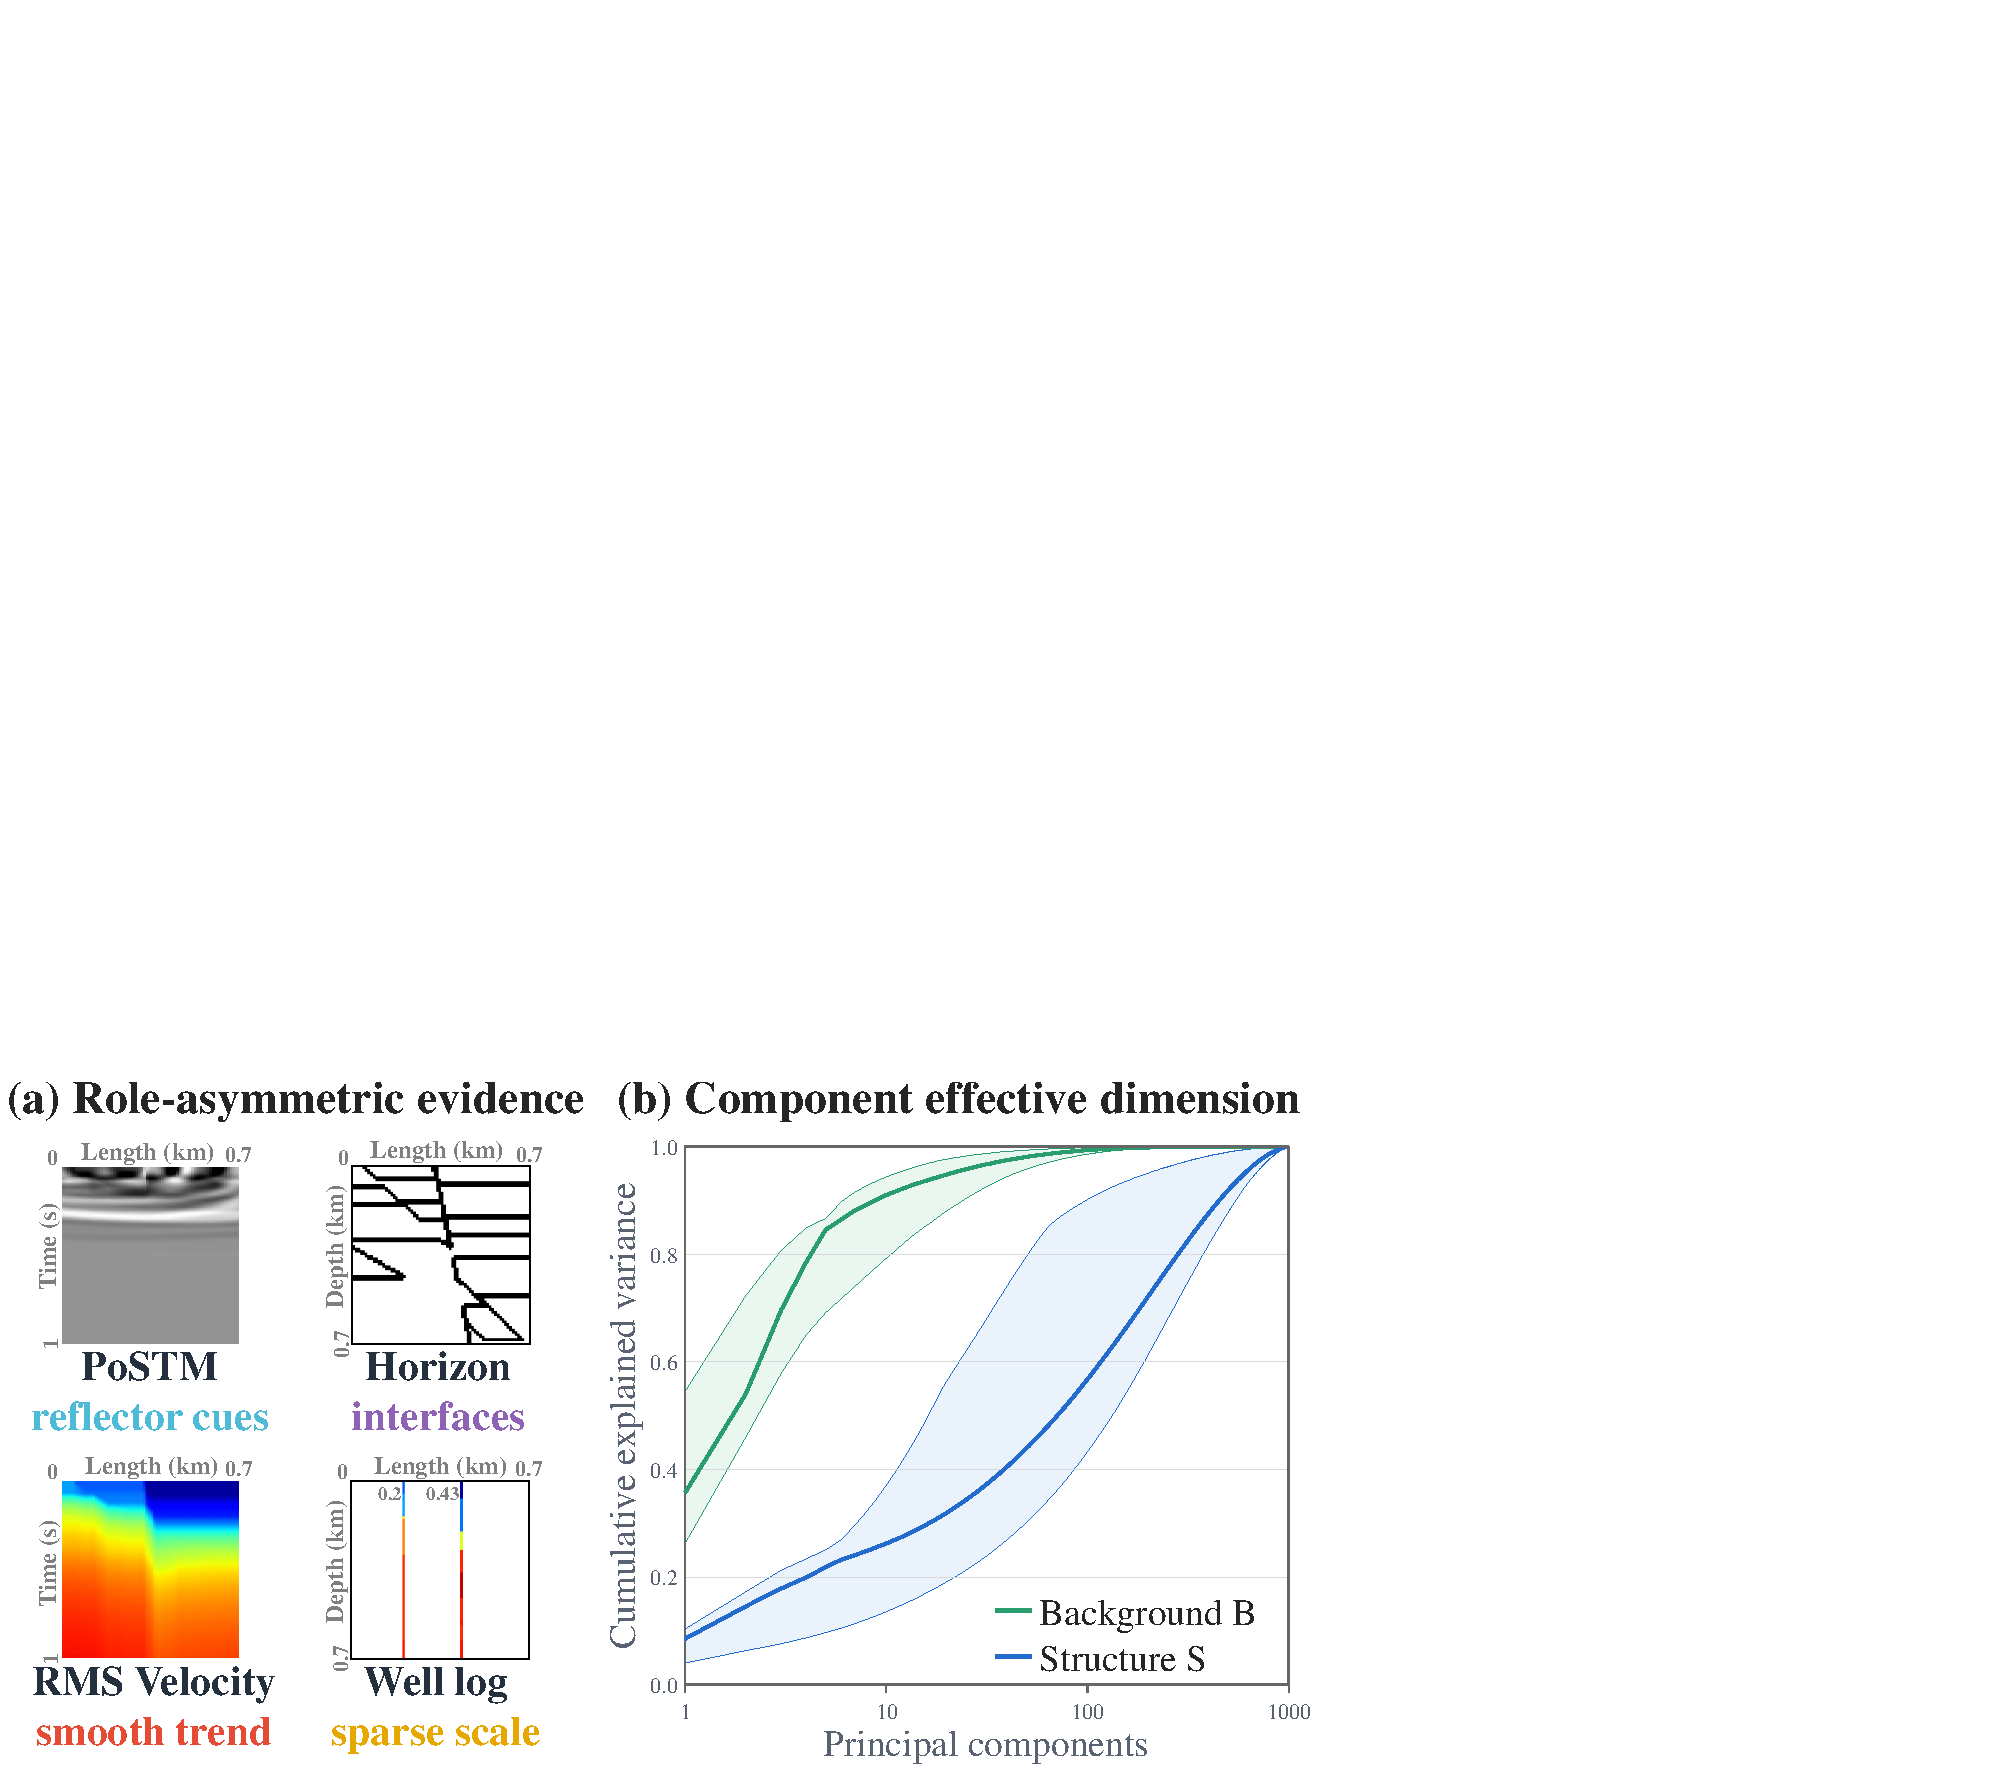
\includegraphics[width=0.98\columnwidth]{figures/aaai/motivation.pdf}
\caption{Data-level evidence for asymmetric conditional complexity. (a) Complementary geometry- and magnitude-oriented modality cues. (b) Cumulative PCA explained-variance curves across eight OpenFWI training subsets: background $B$ concentrates variance in fewer principal directions than structure $S$ (median effective rank $4.95$ versus $54.03$).}
\label{fig:motivation}
\end{figure}

\section{Introduction}

Subsurface velocity inversion estimates depth-domain velocity models for migration and structural interpretation \cite{stolt1978migration}. Classical full-waveform inversion (FWI) repeatedly solves the wave equation, but remains sensitive to initialization, acquisition coverage, cycle skipping, and computational cost \cite{tarantola1984inversion,bunks1995multiscale,pratt1998gaussnewton,virieux2009overview}. Learned inverse models amortize this mapping \cite{arayapolo2018deeptomography,yang2019deeplearning,wu2020inversionnet}, and OpenFWI provides large-scale benchmarks across velocity and fault families \cite{deng2022openfwi}. Practical model construction can also use post-stack migrated images (PoSTM), interpreted horizons, RMS velocity, and well logs \cite{stolt1978migration,dix1955velocities,hampson2001multiattribute}: the first two localize interfaces, while the latter constrain smooth trends and absolute scale.

Learned inversion has advanced mainly by changing the estimator applied after observations are assembled: direct encoder-decoders \cite{wu2020inversionnet,deng2022openfwi,najafi2025svinvnet}, physics-informed models \cite{rashtbehesht2022pinn,jin2022upfwi}, and structured forward/inverse representations or latent mappings \cite{feng2024autolinear,gupta2025gfi}. These methods span supervised, physics-coupled, and latent-translation paradigms. Although their estimators differ, they generally retain one organization: a fixed representation feeds a full-field predictor. This is natural for a single waveform input; with heterogeneous observations, it leaves generation responsibility unassigned: which evidence should control which target component?

Generative modeling broadens the expressiveness of this estimator. Diffusion, score-based, and latent diffusion models provide stochastic priors \cite{ho2020ddpm,song2021scorebased,rombach2022ldm}, including posterior sampling for noisy inverse problems \cite{chung2023diffusionposterior}; Flow Matching and rectified flow learn continuous probability transport \cite{lipman2023flowmatching,liu2023rectifiedflow}, related to dynamic transport \cite{benamou2000computational}. Recent seismic applications include velocity synthesis and inversion \cite{wang2024controllable,wang2024wavediffusion,shan2026reddiffeq}. Applied to the full field, however, one generator transports a predictable regional background through the same stochastic path as complex interfaces, faults, and layers. This couples components with different effective dimensions, while scaling the shared estimator neither assigns observations to components nor determines which component requires transport.

To condition these generators, multimodal representation learning typically emphasizes alignment and availability. Contrastive models align paired views \cite{tian2020cmc,radford2021clip}, Symile preserves agreement among arbitrary modality tuples \cite{saporta2024symile}, and HeMIS handles missing observations \cite{havaei2016hemis}; broader surveys organize alignment, fusion, and modality-specificity challenges \cite{baltrusaitis2019multimodal}. These methods answer how observations should be aligned or retained, not which generation responsibility each condition should serve. This distinction remains even with perfectly aligned features: the downstream estimator still handles both components unless generation itself is routed. Compressing heterogeneous evidence into one condition therefore provides no explicit interface between background and residual roles.

Early fusion permits role leakage, while full-field generation assigns one estimator to components of different conditional complexity. RMS velocity and sparse wells constrain much of the smooth background, whereas PoSTM and horizons primarily constrain the geometry of the remaining correction. The former is comparatively concentrated; the latter retains richer structural variability. We call this mismatch an \emph{asymmetry of conditional complexity}. Figure~\ref{fig:motivation} quantifies it using PCA \cite{jolliffe2002pca}: across all eight OpenFWI subsets, background $B$ concentrates variance in fewer directions than structure $S$, with median participation-ratio effective ranks of $4.95$ and $54.03$. This pronounced decomposition-specific degree-of-freedom gap motivates distinct estimator assignments, not simply a larger fused representation.

Frequency separation alone does not resolve the assignment. Oracle residualization creates a target shift: training uses $R_B=V-B$, but inference composes with $\hat B$, introducing a background mismatch $\hat B-B$ absent from supervision. The prediction-relative residual $R_{\hat B}=V-\hat B$ instead models the remaining \emph{structure-bearing variation} and any correction required for exact composition. Reusing $\hat B$ for residual supervision, conditioning, and composition defines \emph{prediction consistency}.

We propose \emph{Physics-Decoupled Background-Guided Residual Flow Matching} (PD-BG-RFM). Physics-decoupled contrastive learning uses subset-aware alignment, training-only wavelet anchors, cross-role separation, and reliability-weighted fusion to construct separate interfaces for background prediction and structural guidance without hard-assigning modalities to routes. The background interface predicts $\hat B$, which defines $V-\hat B$, conditions residual transport with $C_{\mathrm{str}}$, and composes the final estimate. This yields the block-triangular contract $C_{\mathrm{bg}}\mapsto\hat B$ and $(C_{\mathrm{str}},\hat B)\mapsto\hat R$, linking representation roles to generation responsibilities. The interfaces are learned jointly, but dependence flows only from the predicted background into the residual route. We derive exact composition and low-pass identities and characterize when this routing lowers straight-path target energy.

Our contributions are threefold:
\begin{itemize}
\item We identify an asymmetry of conditional complexity and formalize the block-triangular contract $C_{\mathrm{bg}}\mapsto\hat B$ and $(C_{\mathrm{str}},\hat B)\mapsto\hat R$, whose one-way background-to-residual dependence is instantiated by physics-decoupled contrastive learning.
\item We introduce prediction-consistent residual Flow Matching, reusing one background prediction for residual supervision, vector-field conditioning, and final composition. This shared reference removes background mismatch from composition error by construction.
\item We derive exact composition-consistency and low-pass-burden identities and prove a necessary-and-sufficient condition for residual transport to have lower straight-path target energy than full-field transport.
\end{itemize}
On globally held-out OpenFWI examples, PD-BG-RFM achieves the best matched-input RMSE, SSIM, and high-frequency MAE with only 10.6M parameters. This compact design assigns deterministic prediction to the background and residual transport to the prediction-relative correction. Controlled ablations and branch-specific diagnostics test whether its performance and efficiency follow from the proposed condition interfaces and responsibility allocation.

\begin{figure*}[t]
\centering
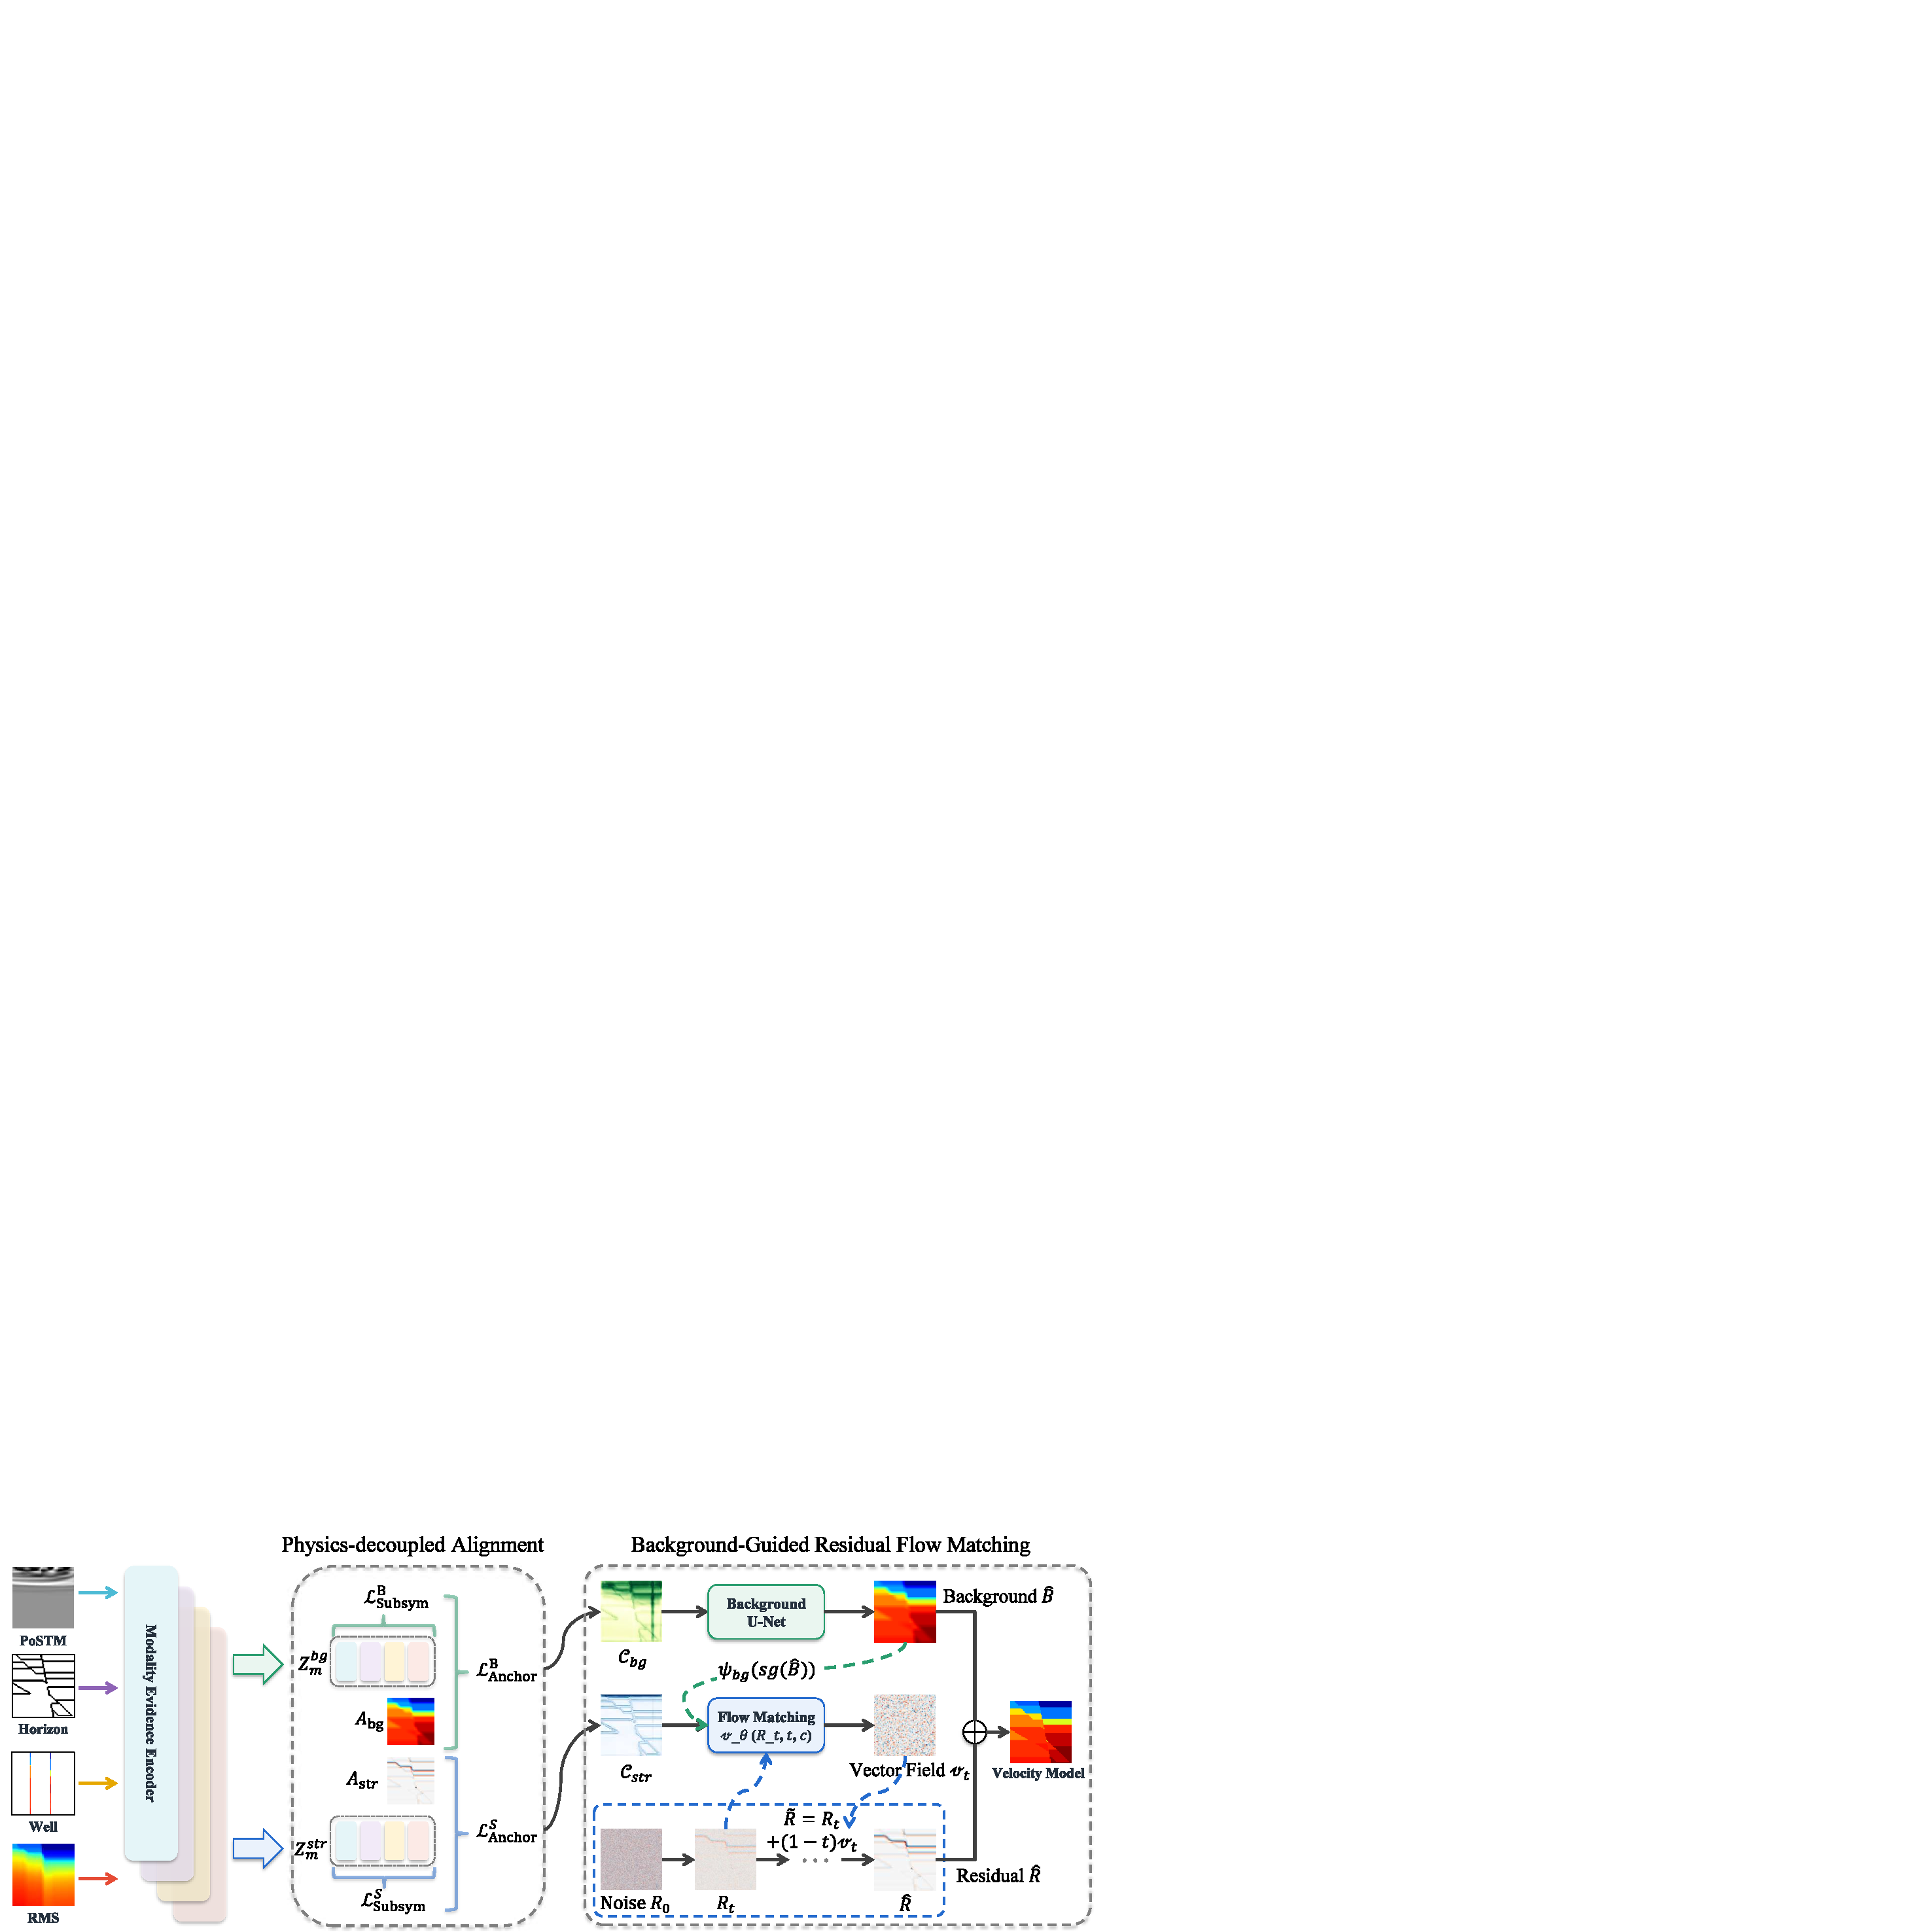
\includegraphics[width=0.98\textwidth]{figures/aaai/method_overview.pdf}
\caption{PD-BG-RFM and its physics-decoupled condition contract. Dashed orange paths provide training supervision; solid paths form inference. The background prediction defines the residual target, conditions transport, and composes the output.}
\label{fig:method-overview}
\end{figure*}

\section{Method}

\subsection{The Physics-Decoupled Condition Contract}
Let $X_\Omega=\{x_m:m\in\Omega\}$ be the observed subset, with $\Omega\subseteq\mathcal M$ and $\mathcal M=\{\mathrm{PoSTM},\mathrm{Horizon},\mathrm{RMS},\mathrm{Well}\}$, and let $V\in\mathbb R^{H\times W}$ be the target velocity model. We assign deterministic prediction to background velocity and generative transport to the remaining structure-bearing variation. PoSTM and horizons predominantly localize geometry, whereas RMS velocity and wells calibrate magnitude \cite{stolt1978migration,dix1955velocities,hampson2001multiattribute}; these are tendencies, not a hard modality partition, so both roles encode every available modality. We implement $P_L$ as linear stride-one average pooling and set $P_H=I-P_L$:
\begin{equation}
B=P_L(V),\qquad S=P_H(V),\qquad V=B+S.
\label{eq:frequency-view}
\end{equation}
$S$ is the complementary component induced by smoothing and is used for training and diagnosis. The transported variable is instead the prediction-relative residual $R_{\hat B}=V-\hat B$, which generalizes $S$ by including the background correction required for exact composition.

\paragraph{Definition 1 (Physics-decoupled condition contract).}
Let $b$ and $r$ denote the background and residual variables, and let $\psi_{\mathrm{bg}}$ be a learned convolutional embedding of a background field. We define the contract as the following block-triangular conditional factorization:
\begin{equation}
\begin{aligned}
(C_{\mathrm{bg}},C_{\mathrm{str}})&=E_\phi(X_\Omega),\\
p_{\mathrm{PD}}(b,r\mid X_\Omega)
&=\delta_{f_{\mathrm{bg}}(C_{\mathrm{bg}})}(b)
\,p_\theta(r\mid C_{\mathrm{str}},\psi_{\mathrm{bg}}(b)).
\end{aligned}
\label{eq:asymmetric-factorization}
\end{equation}
The estimate is $\hat V=\hat B+\hat R$, where $\hat B=f_{\mathrm{bg}}(C_{\mathrm{bg}})$ and $\hat R\sim p_\theta(\,\cdot\mid C_{\mathrm{str}},\psi_{\mathrm{bg}}(\hat B))$. Thus $C_{\mathrm{bg}}$ is the interface for deterministic background prediction, while $C_{\mathrm{str}}$ and the predicted background jointly condition structure-bearing residual generation. The one-way dependence from the background route to the residual route makes the factorization block triangular, without imposing a hard modality partition inside $E_\phi$. The Dirac measure encodes this architectural point-estimator assignment, not a degenerate true posterior, frequency--uncertainty equivalence, or identifiable representation. Figure~\ref{fig:method-overview} summarizes the contract and computation graph.

\subsection{Instantiating the Condition Contract}
In Definition~1, $E_\phi$ is the complete condition-learning stack: modality subencoders, role-aware fusion, and internal role adapters. Each $\mathcal E_{\phi,m}(x_m)=(Z_m^{\mathrm{bg}},Z_m^{\mathrm{str}},r_m)$ uses a convolutional backbone on the velocity grid, lightweight $1\times1$ role heads, and a reliability head $r_m=(r_m^{\mathrm{bg}},r_m^{\mathrm{str}})$. Physics-decoupled contrastive learning calibrates these features and routes while retaining every modality in both roles. The fusion and adapters below therefore belong to $E_\phi$, rather than forming extra condition modules, and are optimized jointly as one condition mapping. A training-only auxiliary separation regularizer does not create a third interface or enter either generator; full details appear in Appendix~\ref{app:condition-objective}.

Suppressing the sample index, let $a_m\in\{0,1\}$ and $q_m\in[0,1]$ denote availability and external quality, with $\Omega=\{m:a_m=1\}$. Role-aware fusion forms
\begin{align}
\bar C_k
&=\sum_{m\in\Omega}w_m^k Z_m^k,
\qquad k\in\{\mathrm{bg},\mathrm{str}\},\nonumber\\
C_{\mathrm{bg}}&=\bar C_{\mathrm{bg}},\qquad
C_{\mathrm{str}}=g_{\mathrm{str}}(\bar C_{\mathrm{str}}).
\label{eq:reliability-fusion}
\end{align}
Here the background adapter is the identity, whereas $g_{\mathrm{str}}$ is a lightweight spatial adapter that produces the generator's structural condition; the two interfaces may have different channel counts. The normalized $w_m^k$ combines availability $a_m$, externally supplied quality $q_m$, and predicted role reliability $r_m^k$, assigning zero weight to unavailable modalities. In our OpenFWI protocol $q_m=a_m$, and no target-derived statistic enters fusion; Appendix~\ref{app:condition-objective} restores the sample index and gives the complete normalization.

Training-only Haar anchors $A_{\mathrm{bg}}=W_L(V)$ and $A_{\mathrm{str}}=W_H(V)$ \cite{mallat1989theory} calibrate the two roles: the former is the resized approximation band and the latter combines detail bands. They differ from the average-pooled background target $B$ and are unavailable at inference. The active condition objective is
\begin{align}
\mathcal L_C
={}&\mathcal L_{\mathrm{subsym}}^{\mathrm{bg}}
 +\mathcal L_{\mathrm{subsym}}^{\mathrm{str}}+\lambda_A\mathcal L_A
 +\lambda_{\mathrm{bg,str}}\mathcal L_{\mathrm{bg,str}}^{\perp}
\nonumber\\
&+\lambda_{\mathrm{aux}}\mathcal L_{\mathrm{aux}}^{\perp}
 +\lambda_Q\mathcal L_{\mathrm{rel}}.
\label{eq:condition-loss}
\end{align}
Subset-Symile \cite{saporta2024symile} encourages joint alignment among each observed modality tuple and its role anchor. The remaining terms specialize these features for the two routes: $\mathcal L_A$ provides symmetric anchor calibration \cite{chen2020simclr}, $\mathcal L_{\mathrm{bg,str}}^{\perp}$ suppresses cross-role leakage through shared/private subspace separation \cite{bousmalis2016domain}, and $\mathcal L_{\mathrm{rel}}$ regularizes fusion toward role-specific priors. The auxiliary term further separates representations without defining another interface. Together, the objective addresses tuple alignment, semantic calibration, role separation, and subset-aware fusion. Appendix~\ref{app:condition-objective} defines every term, diagnostic-only weights, and routing normalization; joint training uses $\lambda_C=0.01$.


\begin{algorithm}[!b]
	\caption{Training procedure for PD-BG-RFM under the backward contract}
	\label{alg:pdbg-rfm}
	\textbf{Input}: batch $\mathcal B=(X_\Omega,V,a,q)$\\
	\textbf{Parameters}: $\Theta=(\phi,\omega_{\mathrm{bg}},\theta)$\\
	\textbf{Output}: updated parameters $\Theta$
	\begin{algorithmic}[1]
		\STATE \textbf{I. Learn physics-decoupled conditions.}
		\STATE $\{Z_m^{\mathrm{bg}},Z_m^{\mathrm{str}},r_m\}_{m\in\Omega}\gets\{\mathcal E_{\phi,m}(x_m)\}_{m\in\Omega}$.
		\STATE $(\bar C_{\mathrm{bg}},\bar C_{\mathrm{str}})\gets\operatorname{Fuse}_{a,q,r}(\{Z_m^{\mathrm{bg}},Z_m^{\mathrm{str}}\}_{m\in\Omega})$.
		\STATE $C_{\mathrm{bg}}\gets\bar C_{\mathrm{bg}}$; $C_{\mathrm{str}}\gets g_{\mathrm{str}}(\bar C_{\mathrm{str}})$.
		\STATE $(A_{\mathrm{bg}},A_{\mathrm{str}})\gets(W_L(V),W_H(V))$; compute $\mathcal L_C$ by Eq.~\ref{eq:condition-loss}.
		\STATE \textbf{II. Predict background velocity deterministically.}
		\STATE $\hat B\gets f_{\mathrm{bg}}(C_{\mathrm{bg}})$; compute $\mathcal L_{\mathrm{bg}}$ by Eq.~\ref{eq:background-loss}.
		\STATE $\bar B\gets\operatorname{sg}[\hat B]$; $R_{\hat B}\gets V-\bar B$.
		\STATE \textbf{III. Transport the prediction-consistent residual.}
		\STATE Sample $t\sim\mathcal U(0,1)$ and $\xi\sim\mathcal N(0,I)$.
		\STATE $c\gets[C_{\mathrm{str}};\psi_{\mathrm{bg}}(\bar B)]$; $R_t\gets(1-t)\xi+tR_{\hat B}$.
		\STATE $u_t\gets R_{\hat B}-\xi$; $\widehat u_t\gets v_\theta(R_t,t,c)$.
		\STATE $\widetilde R\gets R_t+(1-t)\widehat u_t$; compute $\mathcal L_R$ by Eq.~\ref{eq:residual-loss}.
		\STATE \textbf{IV. Optimize under the backward contract.}
		\STATE $\mathcal L\gets\mathcal L_R+\mathcal L_{\mathrm{bg}}+\lambda_C\mathcal L_C$.
		\STATE $\Theta\gets\operatorname{OptStep}(\Theta,\nabla_\Theta\mathcal L)$.
		\STATE \textbf{return} $\Theta$
	\end{algorithmic}
\end{algorithm}


\subsection{Background-Guided Residual Flow Matching}
A full-resolution U-Net \cite{ronneberger2015unet} with parameters $\omega_{\mathrm{bg}}$ deterministically predicts $\hat B=f_{\mathrm{bg}}(C_{\mathrm{bg}})$ on the same spatial grid as $V$, under
\begin{equation}
\mathcal L_{\mathrm{bg}}
=
\|\hat B-P_L(V)\|_1+\lambda_{\mathrm{bg},2}\|\hat B-P_L(V)\|_2^2.
\label{eq:background-loss}
\end{equation}
The prediction is reused throughout the pipeline: it defines residual supervision, joins $C_{\mathrm{str}}$ as context, and is added back for final composition. We therefore define
\begin{equation}
R_{\hat B}=V-\hat B,
\label{eq:prediction-consistent-residual}
\end{equation}
rather than the oracle residual $R_B=V-B$. Using the same $\hat B$ for supervision, context, and composition aligns the residual task encountered during training and inference. We call this construction \emph{prediction-consistent residual transport}; Theorem~1 characterizes it.


\begin{table*}[t]
	\centering
	% PD-BG-RFM values come from the verified global-held-out final-checkpoint artifact.
	% AAAI permits 9pt tables when the normal 10pt size does not fit.
	\small
	\setlength{\tabcolsep}{2pt}
	\begin{tabular*}{\textwidth}{@{\extracolsep{\fill}}c c c c c c c c c@{}}
		\toprule
		Dataset & Metric & InversionNet & VelocityGAN & UPFWI & Auto-Linear & \shortstack{Invertible\\X-Net} & \shortstack{Latent U-Net\\(Large)} & \textbf{PD-BG-RFM} \\
		\midrule
		\multicolumn{2}{c}{\shortstack{Method paper}} & \multicolumn{2}{c}{\shortstack{NeurIPS 2022\\\cite{deng2022openfwi}}} & \shortstack{ICLR 2022\\\cite{jin2022upfwi}} & \shortstack{ICML 2024\\\cite{feng2024autolinear}} & \multicolumn{2}{c}{\shortstack{ICLR 2025\\\cite{gupta2025gfi}}} & \shortstack{\textbf{Ours}} \\
		\midrule
		& MAE$\downarrow$ & 0.0143 & 0.0118 & 0.0621 & \underline{0.0081} & 0.0159 & \textbf{0.0060} & 0.0087 \\
		FlatVel-A & RMSE$\downarrow$ & 0.0257 & 0.0178 & 0.1233 & 0.0224 & 0.0235 & \textbf{0.0098} & \underline{0.0138} \\
		& SSIM$\uparrow$ & 0.9909 & 0.9916 & 0.9565 & 0.9888 & 0.9917 & \textbf{0.9967} & \underline{0.9961} \\
		\addlinespace[2pt]
		& MAE$\downarrow$ & 0.0304 & 0.0329 & 0.0677 & 0.0467 & 0.0233 & \underline{0.0187} & \textbf{0.0168} \\
		FlatVel-B & RMSE$\downarrow$ & 0.0680 & 0.0807 & 0.1493 & 0.1229 & 0.0557 & \underline{0.0536} & \textbf{0.0274} \\
		& SSIM$\uparrow$ & 0.9356 & 0.9521 & 0.8874 & 0.9044 & 0.9769 & \underline{0.9809} & \textbf{0.9877} \\
		\midrule
		& MAE$\downarrow$ & 0.0590 & 0.0482 & 0.0805 & 0.0738 & 0.0386 & \underline{0.0320} & \textbf{0.0099} \\
		CurveVel-A & RMSE$\downarrow$ & 0.1231 & 0.1034 & 0.1411 & 0.1371 & 0.0807 & \underline{0.0749} & \textbf{0.0155} \\
		& SSIM$\uparrow$ & 0.8345 & 0.8624 & 0.8443 & 0.8057 & 0.9135 & \underline{0.9273} & \textbf{0.9962} \\
		\addlinespace[2pt]
		& MAE$\downarrow$ & 0.1448 & 0.1268 & 0.1777 & 0.1820 & 0.0932 & \underline{0.0824} & \textbf{0.0219} \\
		CurveVel-B & RMSE$\downarrow$ & 0.3111 & 0.2618 & 0.3179 & 0.3242 & 0.2067 & \underline{0.2020} & \textbf{0.0374} \\
		& SSIM$\uparrow$ & 0.6630 & 0.7111 & 0.6614 & 0.6169 & 0.8076 & \underline{0.8156} & \textbf{0.9878} \\
		\midrule
		& MAE$\downarrow$ & \underline{0.0128} & 0.0868 & 0.0876 & 0.0164 & 0.0396 & 0.0206 & \textbf{0.0088} \\
		FlatFault-A & RMSE$\downarrow$ & 0.0351 & 0.1485 & 0.2060 & 0.0510 & 0.0586 & \underline{0.0323} & \textbf{0.0199} \\
		& SSIM$\uparrow$ & 0.9834 & 0.9313 & 0.9340 & 0.9701 & 0.9826 & \underline{0.9910} & \textbf{0.9934} \\
		\addlinespace[2pt]
		& MAE$\downarrow$ & 0.0965 & 0.0925 & 0.1416 & 0.1208 & 0.0627 & \underline{0.0619} & \textbf{0.0175} \\
		FlatFault-B & RMSE$\downarrow$ & 0.1636 & 0.1600 & 0.2220 & 0.1903 & \underline{0.1203} & 0.1228 & \textbf{0.0324} \\
		& SSIM$\uparrow$ & 0.7323 & 0.7476 & 0.6937 & 0.6868 & \underline{0.8532} & 0.8515 & \textbf{0.9909} \\
		\midrule
		& MAE$\downarrow$ & 0.0303 & 0.0258 & 0.0500 & 0.0277 & 0.1324 & \underline{0.0180} & \textbf{0.0094} \\
		CurveFault-A & RMSE$\downarrow$ & 0.0766 & 0.0606 & 0.0966 & 0.0781 & 0.1851 & \underline{0.0409} & \textbf{0.0200} \\
		& SSIM$\uparrow$ & 0.9448 & 0.9613 & 0.9495 & 0.9426 & 0.9316 & \underline{0.9800} & \textbf{0.9936} \\
		\addlinespace[2pt]
		& MAE$\downarrow$ & 0.1705 & 0.1571 & 0.3452 & 0.1791 & \underline{0.1207} & 0.1235 & \textbf{0.0260} \\
		CurveFault-B & RMSE$\downarrow$ & 0.2635 & 0.2427 & 0.5010 & 0.2640 & \underline{0.1961} & 0.2036 & \textbf{0.0559} \\
		& SSIM$\uparrow$ & 0.6137 & 0.5996 & 0.3941 & 0.5672 & \underline{0.7116} & 0.6930 & \textbf{0.9859} \\
		\midrule
		\multicolumn{2}{c}{Total Params} & 24.41M & 25.59M & 19.00M & 35.45M & 26.06M & 34.96M & \textbf{10.6M} \\
		\bottomrule
	\end{tabular*}
	\caption{Source-native OpenFWI results across two inversion paradigms: waveform-based inversion and multimodal constraint integration. Each method is evaluated in its native observation and evaluation setting. Bold and underlined values rank first and second within each metric row.}
	\label{tab:main-comparison}
\end{table*}

\paragraph{Theorem 1 (Characterization of prediction-consistent residual transport).}
Let $P_L$ be linear, $P_H=I-P_L$, $B=P_L(V)$, and $\hat V=\hat B+\hat R$. Then prediction-consistent residual transport has the following properties.

\textit{(i) Composition consistency.}
The prediction-consistent and oracle-residual errors are, respectively,
\begin{equation}
\begin{aligned}
\hat V-V&=\hat R-R_{\hat B},
&&R_{\hat B}=V-\hat B,\\
\hat V-V&=(\hat B-B)+(\hat R-R_B),
&&R_B=V-B.
\end{aligned}
\label{eq:composition-consistent}
\end{equation}
The first identity makes final error equal to residual estimation error; the oracle construction retains the additive background mismatch $\hat B-B$.

\textit{(ii) Low-pass burden identity.}
The residual target's low-pass content is exactly determined by the background correction and the high-pass detail retained by the background prediction:
\begin{equation}
P_L(R_{\hat B})=(B-\hat B)+P_H(\hat B).
\label{eq:low-frequency-burden}
\end{equation}
Thus the residual's low-pass response is generally nonzero and should be matched to its target rather than suppressed.
\textit{(iii) Straight-path transport energy.}
For fixed $C=(C_{\mathrm{str}},\hat B)$, $V\mapsto R_{\hat B}$ is a unit-Jacobian translation and preserves differential entropy when the relevant densities and entropies exist (Appendix~\ref{app:residual-proofs}). This local invariance does not compare $p(B\mid C_{\mathrm{bg}})$ with $p(R_{\hat B}\mid C_{\mathrm{str}},\hat B)$; the two responsibilities use different conditions and targets. The measurable transport effect is instead characterized exactly below. Vectorize the fields to $d=HW$ dimensions, assume finite second moments, and let $\xi\sim\mathcal N(0,I_d)$ be independent of $(V,C)$. The straight-path targets $u_V=V-\xi$ and $u_R=R_{\hat B}-\xi$ satisfy
\begin{equation}
\mathbb E\|u_R\|_2^2<\mathbb E\|u_V\|_2^2
\iff
\mathbb E\|V-\hat B\|_2^2<\mathbb E\|V\|_2^2.
\label{eq:transport-condition}
\end{equation}
The theorem exactly characterizes the target induced by Definition~1 and provides a necessary-and-sufficient condition for lower straight-path target energy; it does not require representation identifiability or claim that translation alone lowers entropy. The energy comparison is specific to the stated normalized coordinates and Gaussian base. Its proof is given \ifaaaiwithappendix in Appendix~\ref{app:residual-proofs}\else in the supplementary material\fi.

We transport directly on the velocity grid with an identity codec. During optimization, $\bar B=\operatorname{sg}[\hat B]$ equals $\hat B$ in the forward pass but blocks residual-loss gradients, so only backward responsibility changes. The residual U-Net receives the structural condition and a separate convolutional background embedding, $c=[C_{\mathrm{str}};\psi_{\mathrm{bg}}(\bar B)]$. For $t\sim\mathcal U(0,1)$ and $\xi\sim\mathcal N(0,I)$, the linear path and Flow Matching objective are
We transport directly on the velocity grid with an identity codec. During optimization, $\bar B=\operatorname{sg}[\hat B]$ equals $\hat B$ in the forward pass but blocks residual-loss gradients, so only backward responsibility changes. The residual U-Net receives the structural condition and a separate convolutional background embedding, $c=[C_{\mathrm{str}};\psi_{\mathrm{bg}}(\bar B)]$. For $t\sim\mathcal U(0,1)$ and $\xi\sim\mathcal N(0,I)$, the linear path and Flow Matching objective are
\begin{equation}
\begin{aligned}
R_t&=(1-t)\xi+tR_{\hat B},&
u_t&=R_{\hat B}-\xi,\\
\mathcal L_{\mathrm{FM}}
&=\mathbb E_{X_\Omega,V,t,\xi}
\bigl[\|v_\theta(R_t,t,c)-u_t\|_2^2\bigr].
\end{aligned}
\label{eq:fm-objective}
\end{equation}
This objective learns a conditional vector field that transports the Gaussian base toward prediction-relative residuals, rather than toward full velocity models.
The parameters $\theta$ include $\psi_{\mathrm{bg}}$ and the U-Net vector field $v_\theta$, whose residual blocks use feature-wise linear modulation (FiLM) \cite{perez2018film} by $c$ and the time embedding. The one-step endpoint estimate and residual objective are
\begin{equation}
\begin{aligned}
\widetilde R
&=R_t+(1-t)v_\theta(R_t,t,c),\\
\mathcal L_R
&=\mathcal L_{\mathrm{FM}}
+\lambda_{\mathrm{rec}}\|\bar B+\widetilde R-V\|_1\\
&\quad+\lambda_{L}\|P_L(\widetilde R)-P_L(R_{\hat B})\|_1.
\end{aligned}
\label{eq:residual-loss}
\end{equation}
The reconstruction term supervises the composed estimate $\bar B+\widetilde R$, while the final term matches the actual residual target's low-pass response rather than forcing $P_L(\widetilde R)$ to zero. Neither term requires ODE integration during training.

Joint optimization uses
\begin{equation}
\mathcal L=\mathcal L_R+\mathcal L_{\mathrm{bg}}+\lambda_C\mathcal L_C.
\label{eq:total-loss}
\end{equation}
The three objectives are optimized jointly: $\mathcal L_C$ calibrates routing, $\mathcal L_{\mathrm{bg}}$ supervises deterministic background prediction, and $\mathcal L_R$ trains residual transport. No target-derived quality gate is used.

The directed forward factorization has a corresponding \emph{backward contract}. Let $\omega_{\mathrm{bg}}$ and $\theta$ be the exclusive background- and residual-route parameters. Because every residual use of $\hat B$ is stop-gradient and the exclusive parameters are disjoint,
\begin{equation}
\nabla_{\omega_{\mathrm{bg}}}\mathcal L=\nabla_{\omega_{\mathrm{bg}}}\mathcal L_{\mathrm{bg}},
\qquad
\nabla_{\theta}\mathcal L=\nabla_{\theta}\mathcal L_R.
\label{eq:gradient-contract}
\end{equation}
Thus the background predictor is updated only for its deterministic target, while the residual vector field is updated only for prediction-consistent transport. Equation~\ref{eq:gradient-contract} concerns their exclusive parameters; the shared encoder still couples the routes through role-specific conditions and $\mathcal L_C$.

\paragraph{Corollary 1 (Objective design under prediction consistency).}
Under Definition~1, Theorem~1 motivates four linked choices: directly supervise the background predictor, define residual supervision relative to that prediction, condition the vector field on its stop-gradient embedding, and match rather than suppress residual low-pass content. Equations~\ref{eq:background-loss}, \ref{eq:residual-loss}, and~\ref{eq:gradient-contract} instantiate these choices. The energy condition is assessed by Eq.~\ref{eq:transport-diagnostic}, rather than optimized as another loss.

At inference, PD-BG-RFM receives only $X_\Omega$, forms $(C_{\mathrm{bg}},C_{\mathrm{str}})$, and predicts $\hat B$. It solves the neural ODE \cite{chen2018neuralode} induced by $v_\theta$ under $[C_{\mathrm{str}};\psi_{\mathrm{bg}}(\hat B)]$ and composes its endpoint as $\hat V=\hat B+\hat R$. The path accesses neither $V$, wavelet anchors, $P_L(V)$, nor target-derived quality statistics.

\begin{figure*}[htbp]
	\centering
	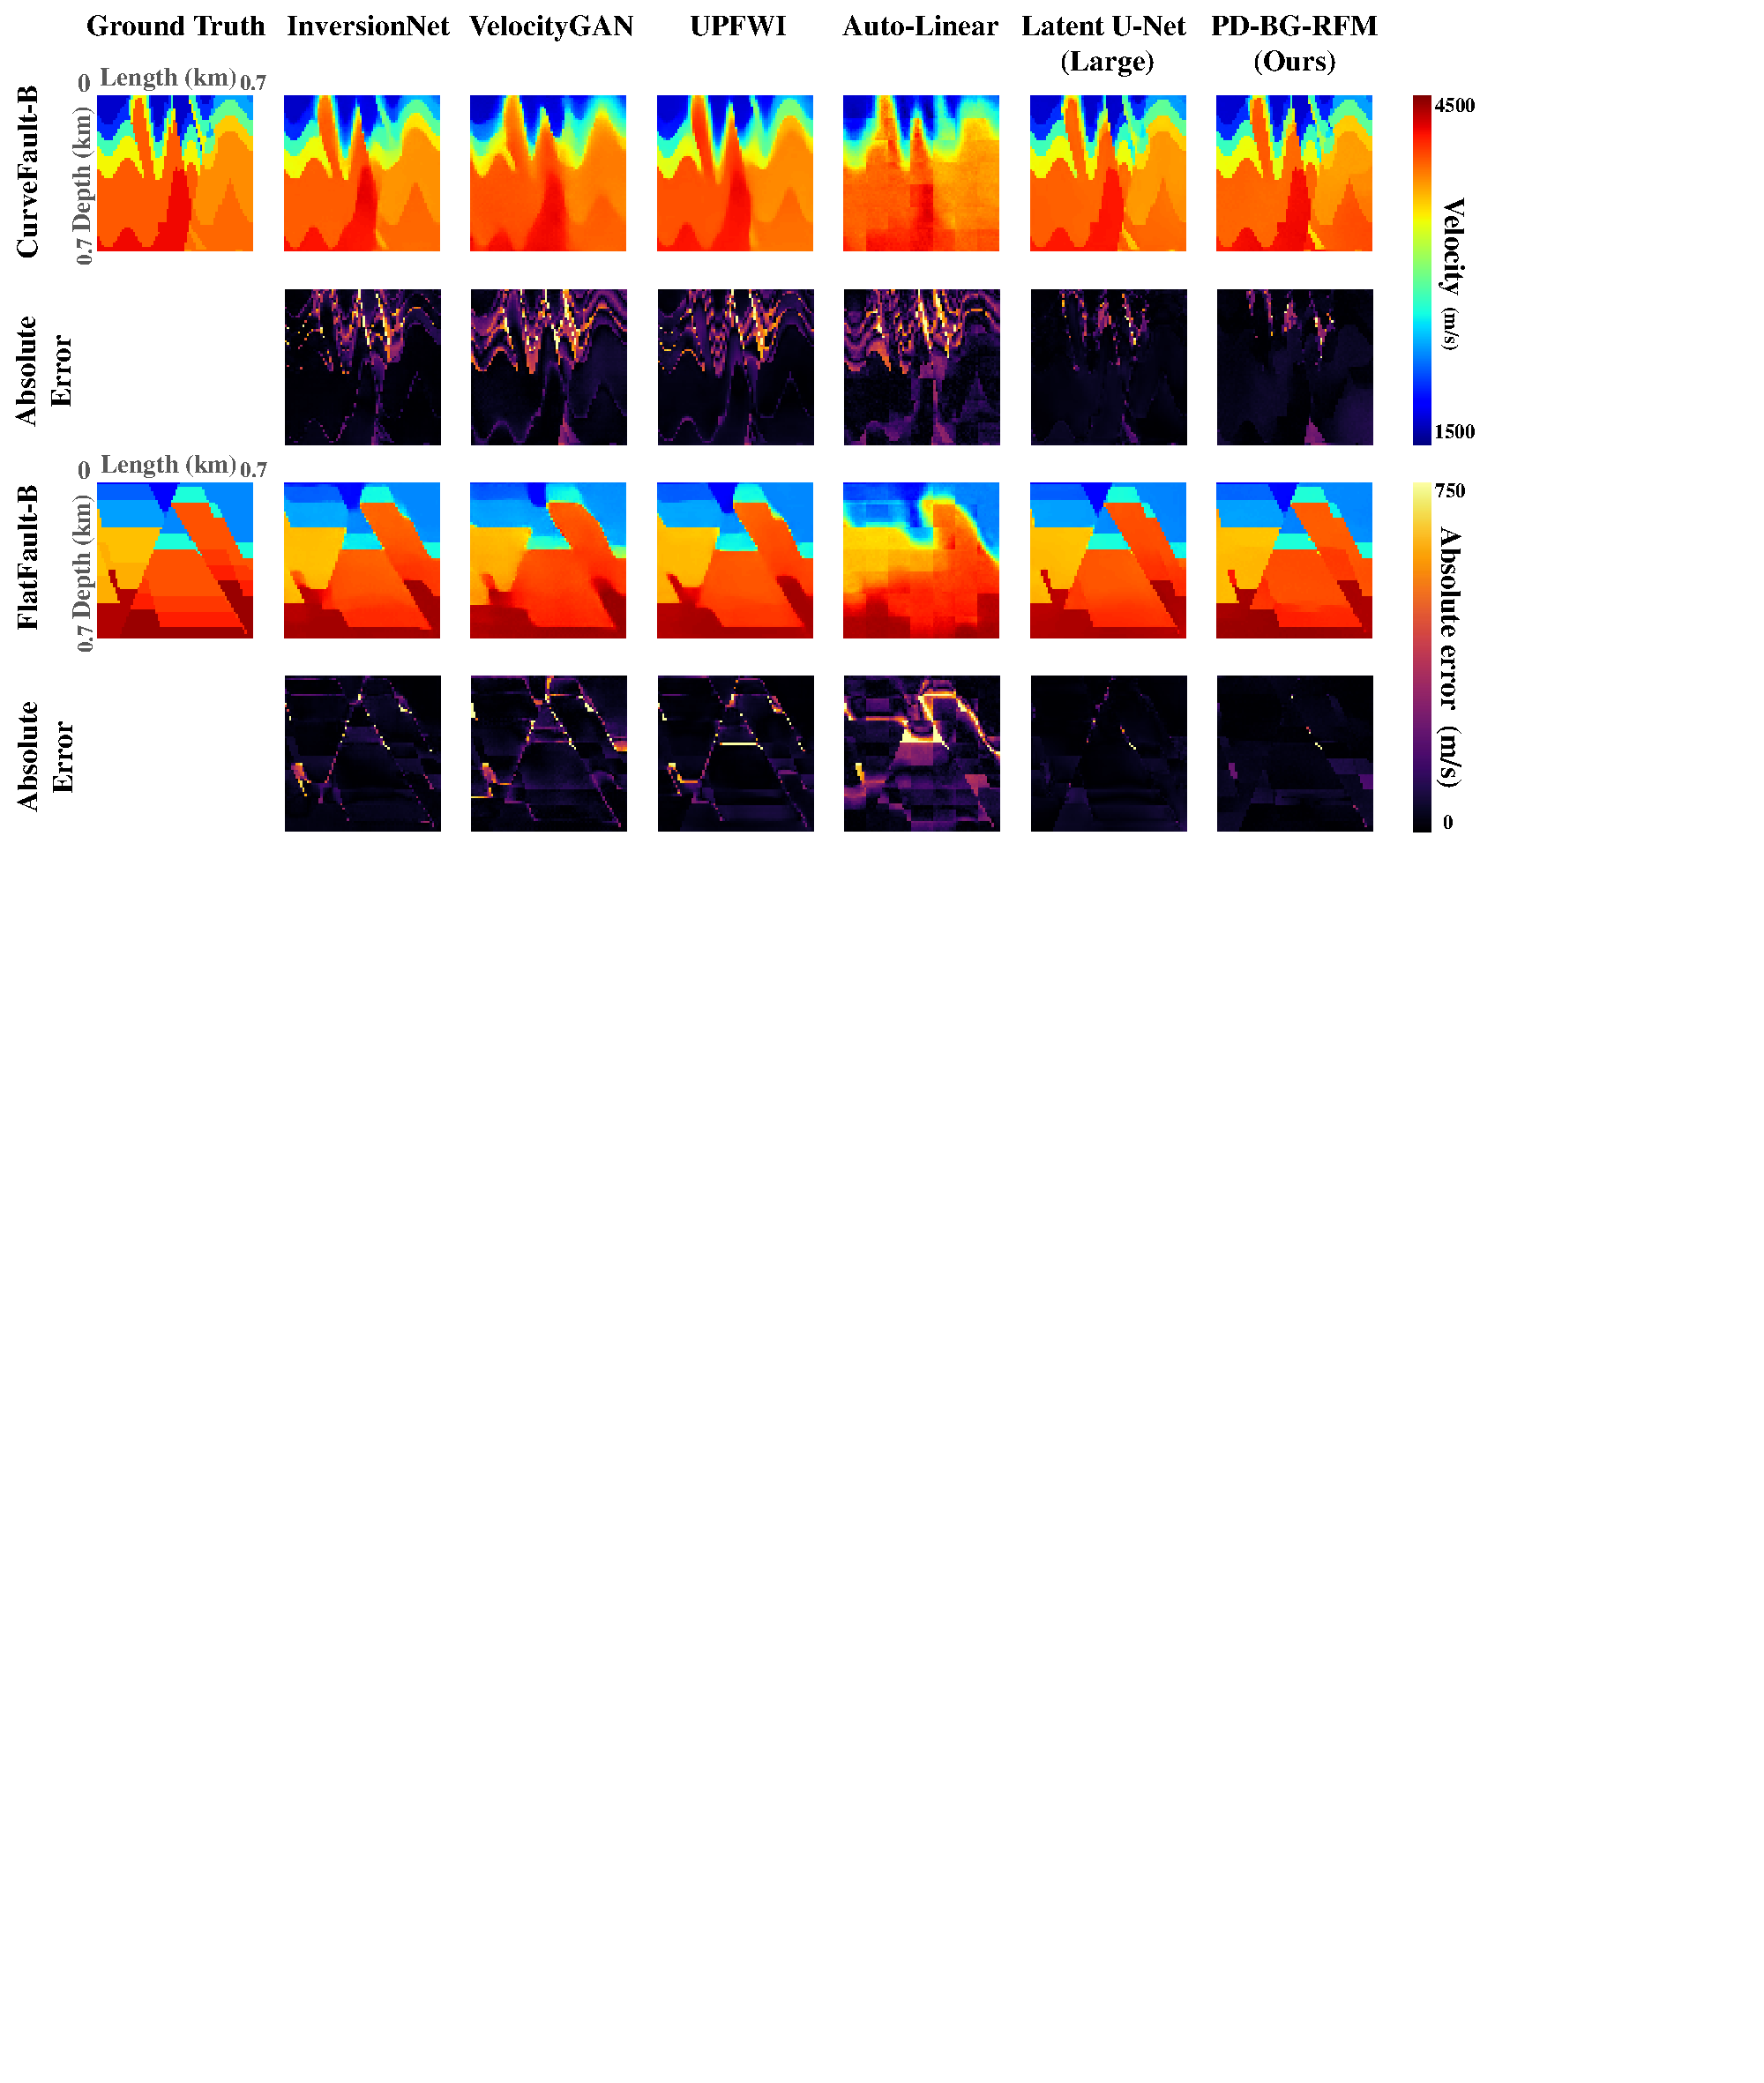
\includegraphics[width=\textwidth]{figures/aaai/qualitative.pdf}
	\caption{Matched-input qualitative results on held-out CurveFault-B and FlatFault-B, highlighting fault and layer-boundary fidelity. Predictions and absolute errors share scales.}
	\label{fig:adapted-qualitative}
\end{figure*}

\section{Experiments}

\subsection{Experimental Setup}
\textbf{Dataset.} OpenFWI is a large-scale public benchmark of synthetic seismic data and two-dimensional velocity models spanning layered, curved, and faulted geology \cite{deng2022openfwi}. We use all eight subsets---FlatVel-A/B, CurveVel-A/B, FlatFault-A/B, and CurveFault-A/B---because their controlled progression from smooth layers to complex faults tests background recovery and structural reconstruction within one benchmark. Our multimodal construction pairs each depth-velocity target with PoSTM, horizon, and RMS-velocity observations and dynamically samples zero to three masked well-log columns. The resulting corpus contains 336,000 records; a deterministic global 7/2/1 split with seed 42 yields 33,600 held-out test records. All matched-input comparisons use the same observations, record identifiers, target normalization, masks, and evaluator.

\textbf{Implementation Details.} PD-BG-RFM uses 16-channel role maps, a background U-Net with 192 hidden channels, and a residual FiLM U-Net with 128 hidden channels conditioned through a 32-channel structural adapter. The complete model is trained end-to-end from random initialization for 100 epochs with AdamW \cite{loshchilov2019decoupled} on four accelerators. Residual inference uses 50 Euler steps, and the model has 10.6M trainable parameters. Matched-input comparisons report sample-averaged MAE, RMSE, SSIM \cite{wang2004ssim}, and low- and high-pass MAE. Wavelet anchors and target-derived quantities are restricted to training or diagnostic analysis and never enter inference. Full architecture, optimization, and metric definitions appear in Appendix~\ref{app:implementation}.

\subsection{Comparison with Existing Methods}
\textbf{Paradigm-level benchmark context.} Table~\ref{tab:main-comparison} contrasts established waveform-based inversion with multimodal constraint integration on OpenFWI, preserving the native observation and evaluation setting of each paradigm. PD-BG-RFM records the strongest value in 21 of 24 subset--metric cells and leads all three metrics on seven of the eight subsets. These results establish multimodal constraint integration as a competitive inversion paradigm across increasingly complex velocity families. Table~\ref{tab:adapted-comparison} then isolates estimator performance under a common multimodal input contract and evaluator. Provenance, scale conversion, parameter counting, and source-protocol details appear in Appendix~\ref{app:benchmark-accounting}.

\begin{table}[t]
		\centering
		\small
		\begin{tabular*}{\columnwidth}{@{\extracolsep{\fill}}l@{\hspace{1.5pt}}c@{\hspace{1.5pt}}c@{\hspace{1.5pt}}c@{\hspace{1.5pt}}c@{\hspace{1.5pt}}c@{\hspace{1.5pt}}c@{}}
			\toprule
			Method & \shortstack{MAE} & \shortstack{RMSE} & \shortstack{SSIM} & \shortstack{$\mathrm{MAE}_L$} & \shortstack{$\mathrm{MAE}_H$} & Params \\
		\midrule
		InversionNet & \underline{0.0149} & 0.0273 & 0.9812 & 0.0180 & \underline{0.0079} & 24.41M \\
		VelocityGAN & 0.0217 & 0.0434 & 0.9727 & 0.0149 & 0.0136 & 25.59M \\
		UPFWI & \textbf{0.0132} & 0.0299 & 0.9895 & \underline{0.0079} & 0.0098 & 19.00M \\
		Auto-Linear & 0.0313 & 0.0593 & 0.9703 & 0.0182 & 0.0229 & 35.47M \\
		\shortstack[l]{Latent U-Net\\(Large)} & 0.0170 & \underline{0.0311} & \underline{0.9910} & \textbf{0.0071} & 0.0134 & 35.12M \\
		\midrule
		\textbf{PD-BG-RFM} & 0.0150 & \textbf{0.0270} & \textbf{0.9913} & 0.0119 & \textbf{0.0065} & \textbf{10.60M} \\
		\bottomrule
		\end{tabular*}
	\caption{Matched-input comparison on 33,600 held-out records. All methods share inputs, split, normalization, and evaluator. Bold and underlined values rank first and second.}
	\label{tab:adapted-comparison}
\end{table}

\textbf{Matched-input estimator comparison.} To complement the paradigm-level comparison, we adapt InversionNet, VelocityGAN, and UPFWI \cite{deng2022openfwi}, Auto-Linear \cite{feng2024autolinear}, and GFI's Latent U-Net (Large) \cite{gupta2025gfi} to the common multimodal input and evaluate all models on identical held-out records with one evaluator. Table~\ref{tab:adapted-comparison} reports their sample-averaged metrics, while Appendix~\ref{app:adapted-accounting} documents implementations and checkpoints. PD-BG-RFM ranks first in RMSE, SSIM, and high-frequency MAE with fewer parameters than every adapted baseline: 10.6M, 44.2\% below the next-smallest model. This efficiency supports asymmetric capacity allocation: deterministic regression handles the background, reserving Flow Matching for the prediction-relative residual characterized by Theorem~1(iii). Figure~\ref{fig:adapted-qualitative} complements these aggregate results with held-out CurveFault-B and FlatFault-B examples. Shared velocity and error scales highlight recovery of faults and layer interfaces while localizing the remaining errors.

\subsection{Condition and Transport Diagnostics}



This section diagnoses two empirical implications of PD-BG-RFM: whether the learned conditions preserve the responsibilities defined by the condition contract and whether prediction-relative residuals satisfy the lower-energy criterion in Theorem~1(iii).
Figure~\ref{fig:condition-contract} tests the representation side of the condition contract. Matched tuples exceed shuffled tuples by median cosine-similarity margins of 0.46 for the background role and 0.35 for the structural role. The fused conditions attain global medians of 0.76 for $\eta_{\mathrm{bg}}$ and 0.66 for $\eta_{\mathrm{str}}$, with cross-role similarity $\chi_{\mathrm{bg,str}}=0.17$. The agreement persists across all eight subsets, providing direct evidence that anchor calibration and role separation survive multimodal fusion.
For a field with $d=HW$ pixels, we measure the normalized straight-path target-energy ratio
\begin{equation}
q_T=\frac{d^{-1}\|V-\hat B\|_2^2+1}{d^{-1}\|V\|_2^2+1}.
\label{eq:transport-diagnostic}
\end{equation}
Here $q_T<1$ is equivalent to the condition in Theorem~1(iii).

\begin{figure}[htbp]
		\centering
		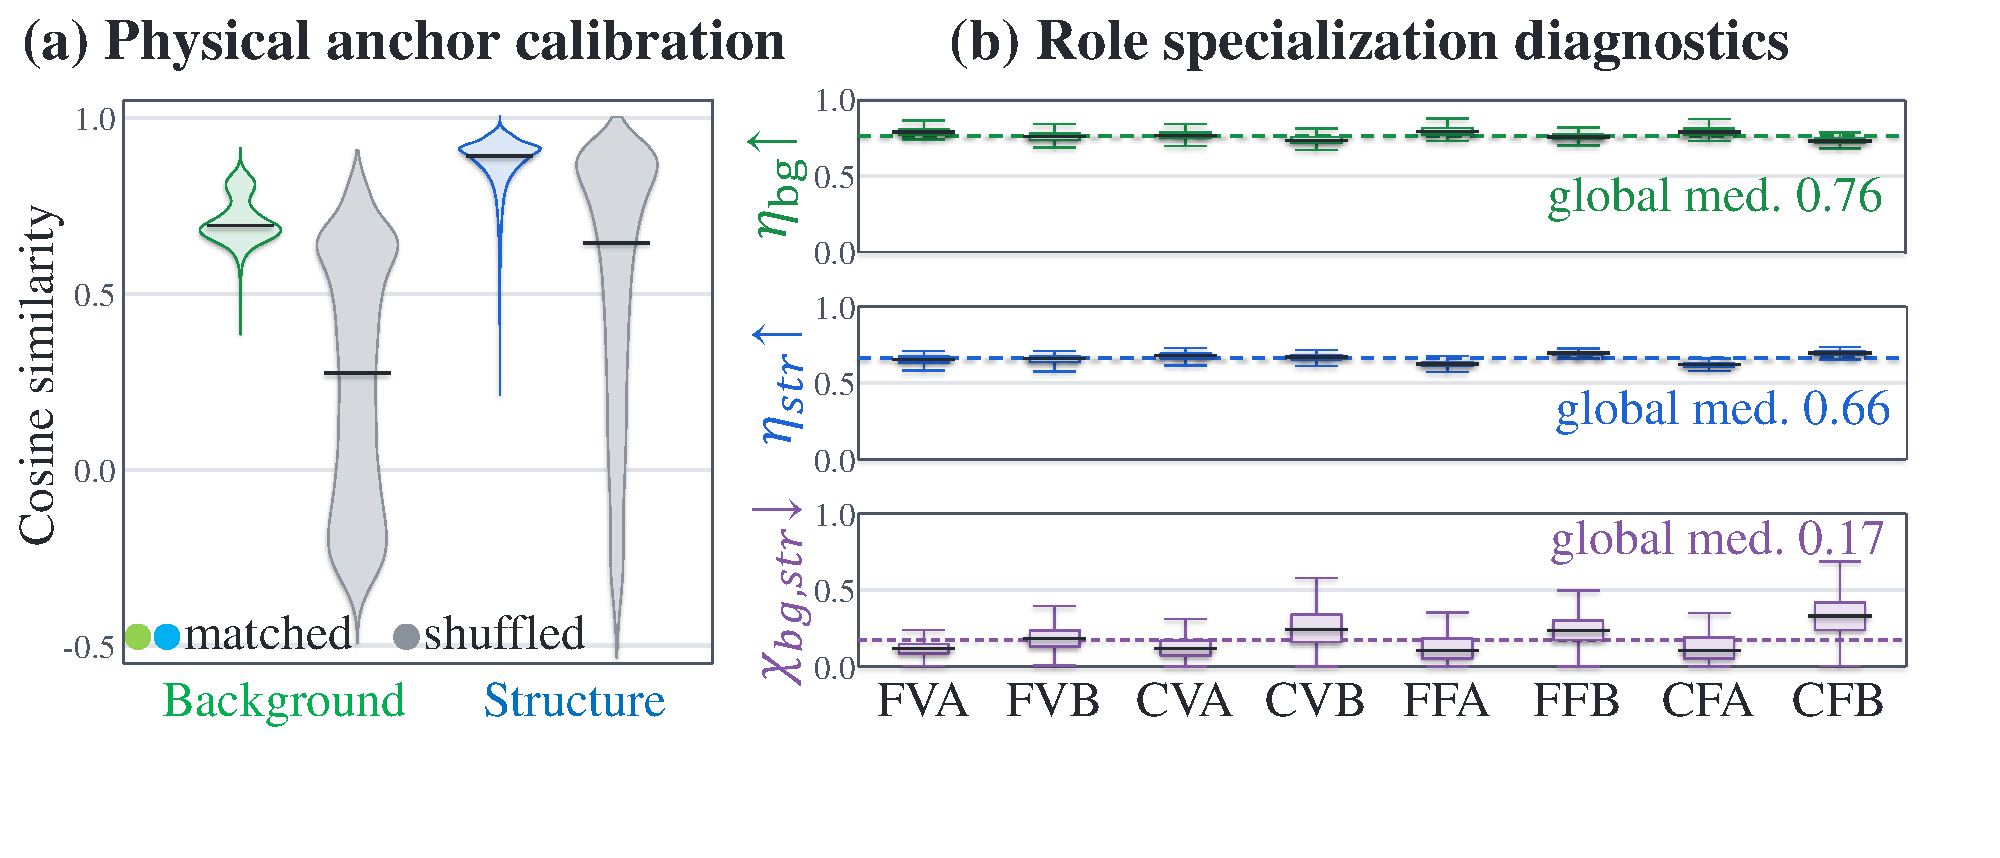
\includegraphics[width=\columnwidth]{figures/aaai/condition_learning.pdf}
	\caption{Condition-routing diagnostics on 33,600 held-out records. (a) Matched--shuffled anchor-similarity margins: 0.46 (background), 0.35 (structural). (b) Role specialization ($\eta_{\mathrm{bg}}$, $\eta_{\mathrm{str}}$) and cross-role similarity ($\chi_{\mathrm{bg,str}}$) by subset. Anchors never enter inference.}
	\label{fig:condition-contract}
\end{figure}

\begin{figure}[htbp]
\centering
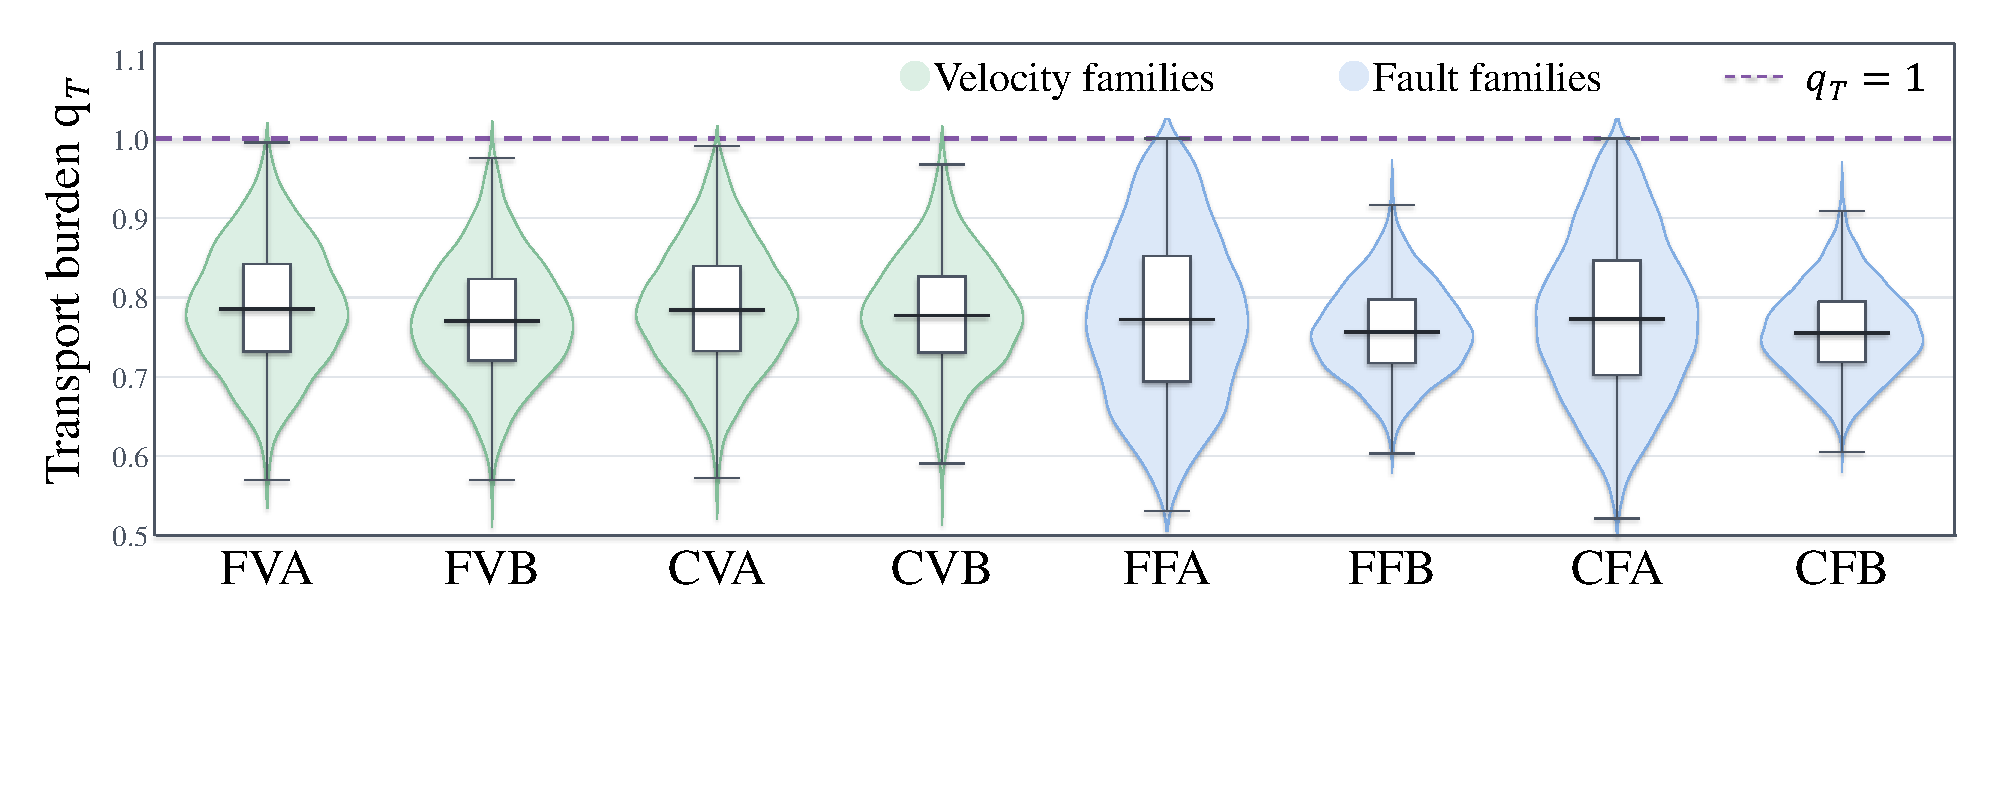
\includegraphics[width=\columnwidth]{figures/aaai/residual_transport.pdf}
\caption{Straight-path target-energy ratio $q_T$ across eight held-out OpenFWI subsets. The dashed line marks $q_T=1$; all 33,600 samples satisfy $q_T<1$.}
\label{fig:residual-transport}
\end{figure}

Figure~\ref{fig:residual-transport} tests this condition on the held-out split. Every one of the 33,600 records satisfies $q_T<1$, with mean 0.772 and bootstrap 95\% confidence interval $[0.771,0.773]$. This corresponds to a 22.8\% average samplewise reduction in normalized straight-path target energy and links the predicted background directly to the intended simplification of residual transport.

Additional condition, background-residual, and missing-modality diagnostics are reported together in Appendix~\ref{app:supplementary-results} under the same held-out protocol.

\subsection{Ablation Study}
\begin{table}[thbp]
	\centering
	\small
	\begin{tabular*}{\columnwidth}{@{\extracolsep{\fill}}l@{\hspace{2.5pt}}c@{\hspace{2.5pt}}c@{\hspace{2.5pt}}c@{\hspace{2.5pt}}c@{\hspace{2.5pt}}c@{}}
		\toprule
		Variant & MAE$\downarrow$ & RMSE$\downarrow$ & SSIM$\uparrow$ & $\mathrm{MAE}_L\downarrow$ & $\mathrm{MAE}_H\downarrow$ \\
		\midrule
		Concat-FM & 0.0225 & 0.0340 & 0.9865 & 0.0189 & \underline{0.0068} \\
		Decoupled-FM & 0.0205 & 0.0320 & 0.9880 & 0.0175 & \underline{0.0068} \\
		Uniform Fusion & \underline{0.0163} & \underline{0.0290} & \underline{0.9898} & \underline{0.0128} & 0.0072 \\
		\shortstack[l]{w/o Prediction\\Consistency} & 0.0190 & 0.0340 & 0.9875 & 0.0156 & 0.0072 \\
		\shortstack[l]{w/o Background\\Context} & 0.0230 & 0.0410 & 0.9820 & 0.0175 & 0.0100 \\
		\textbf{PD-BG-RFM} & \textbf{0.0150} & \textbf{0.0270} & \textbf{0.9913} & \textbf{0.0119} & \textbf{0.0065} \\
		\bottomrule
	\end{tabular*}
	\caption{Controlled ablations on 33,600 held-out records under shared inputs, split, training budget, evaluator, and 50-step Flow Matching inference. Bold and underlined values rank first and second.}
	\label{tab:ablation}
\end{table}

Table~\ref{tab:ablation} follows the construction of PD-BG-RFM under a common protocol. Concat-FM uses one fused condition; Decoupled-FM introduces $C_{\mathrm{bg}}$ and $C_{\mathrm{str}}$ but still generates the full field. Uniform Fusion retains the decoupled architecture but removes reliability weighting. The final two variants remove prediction consistency or the background context $\psi_{\mathrm{bg}}(\hat B)$, respectively. Additional controls appear in Appendix~\ref{app:component-ablations}.


The full model leads all metrics, reducing MAE, RMSE, and low-frequency MAE by 33.3\%, 20.6\%, and 37.0\% over Concat-FM; Decoupled-FM improves SSIM and matches its high-frequency MAE. Replacing $R_{\hat B}$ with $R_B$ degrades all metrics, consistent with Theorem~1(i): composition with $\hat B$ restores the target-shift term $\hat B-B$. Removing $\psi_{\mathrm{bg}}(\hat B)$ raises RMSE by 51.9\% and high-frequency MAE by 53.8\% versus the full model, confirming the prediction's value as vector-field context. Reliability weighting improves all metrics over uniform fusion. These ablations close the contract from role separation through prediction-consistent supervision and background-conditioned transport to composition.

\section{Conclusion}
PD-BG-RFM assigns deterministic prediction to background velocity and generative transport to the prediction-relative residual. Its physics-decoupled condition contract and prediction-consistent reuse of $\hat B$ align residual supervision, vector-field conditioning, and composition. Theory derives exact composition and low-pass identities and proves the condition for lower straight-path target energy. On held-out OpenFWI, the 10.6M-parameter model achieves the best matched-input RMSE, SSIM, and high-frequency MAE. The results support directly predicting well-constrained components and transporting the remaining structure-bearing variation.

\bibliography{references}

\ifaaaiwithappendix
\clearpage
\setcounter{secnumdepth}{1}
\appendix
% Prefix appendix equations, figures, and tables with their lettered section.
\numberwithin{equation}{section}
\numberwithin{figure}{section}
\numberwithin{table}{section}
\section{Theoretical Derivations and Proofs}
\label{app:residual-proofs}
This appendix proves Theorem~1 under its stated assumptions and derives the objective implications summarized by Corollary~1.

\subsection{Proof of Theorem~1}
\paragraph{(i) Composition consistency.}
Let $R_{\hat B}=V-\hat B$ and $\hat V=\hat B+\hat R$. Then
\begin{equation}
\hat V-V=\hat B+\hat R-V=\hat R-(V-\hat B)=\hat R-R_{\hat B}.
\end{equation}
For $R_B=V-B$, adding and subtracting $B$ instead gives
\begin{equation}
\hat V-V=(\hat B-B)+(\hat R-R_B).
\end{equation}
Thus even a perfect oracle-residual prediction leaves the composition error $\hat B-B$, whereas a perfect prediction-consistent residual reconstructs $V$ exactly. This proves Theorem~1(i).

\paragraph{(ii) Low-pass burden identity.}
Let $P_L$ be linear, define $P_H=I-P_L$, and set $B=P_L(V)$. Then
\begin{align}
P_L(V-\hat B)
&=P_L(V)-P_L(\hat B)\\
&=B-\bigl(\hat B-P_H(\hat B)\bigr)\\
&=(B-\hat B)+P_H(\hat B).
\end{align}
This proves Theorem~1(ii). The proof does not assume that $P_L$ is idempotent. In particular, belonging to $\operatorname{Range}(P_L)$ would not imply $P_L(\hat B)=\hat B$ for the stride-one average pool used here. Because the two terms may cancel, the equality is not an additive decomposition of their norms.

\paragraph{(iii) Straight-path transport energy.}
Let $C=(C_{\mathrm{str}},\hat B)$ and assume the conditional densities exist. For fixed $C$, the transform $T_{\hat B}(v)=v-\hat B$ has inverse $T_{\hat B}^{-1}(r)=r+\hat B$ and Jacobian determinant one. The change-of-variables formula gives
\begin{equation}
p_{R_{\hat B}}(r\mid C)=p_V(r+\hat B\mid C).
\end{equation}
Translation invariance of differential entropy then yields $h(R_{\hat B}\mid C)=h(V\mid C)$ whenever these entropies are finite.
This equality concerns only the fixed-condition translation above; it does not compare the conditional complexities of the background and residual responsibilities.

Now let $\xi\sim\mathcal N(0,I_d)$ be independent of $(V,C_{\mathrm{str}},\hat B)$, and define $u_V=V-\xi$ and $u_R=(V-\hat B)-\xi$. Independence and $\mathbb E[\xi]=0$ give
\begin{align}
\mathbb E\|u_R\|^2
&=
\mathbb E\|V-\hat B\|^2+d,\\
\mathbb E\|u_V\|^2
&=
\mathbb E\|V\|^2+d.
\end{align}
Subtracting proves Eq.~\ref{eq:transport-condition}. For a fixed sample $(V,\hat B)$, taking expectation only over $\xi$ gives
\begin{equation}
\frac{\mathbb E_{\xi}[d^{-1}\|u_R\|^2\mid V,\hat B]}
{\mathbb E_{\xi}[d^{-1}\|u_V\|^2\mid V,\hat B]}
=
\frac{d^{-1}\|V-\hat B\|^2+1}{d^{-1}\|V\|^2+1}.
\end{equation}
This is exactly the sample-level diagnostic $q_T$. A value below one verifies the corresponding samplewise energy condition in the stated normalized coordinates. Because an average of ratios is not a ratio of expectations, its test-set mean does not establish the population-level inequality or imply easier learned dynamics, lower conditional entropy, MAE, or RMSE. This proves Theorem~1(iii).

\subsection{Derivation of Corollary~1}
Equation~\ref{eq:composition-consistent} selects the prediction-relative reference used by residual supervision and final composition, while Eq.~\ref{eq:low-frequency-burden} determines the matching target in the low-pass residual term. Together with the conditional factorization in Definition~1, these identities yield the objective construction summarized by Corollary~1 and instantiated in Eqs.~\ref{eq:background-loss}, \ref{eq:residual-loss}, and~\ref{eq:gradient-contract}. Equation~\ref{eq:transport-condition} supplies the post-training diagnostic $q_T$ rather than an additional training term. Thus the corollary maps the theorem to the implemented objective without asserting architectural uniqueness or statistical optimality.


\section{Supplementary Results and Diagnostics}
\label{app:supplementary-results}

\subsection{Extended Qualitative Comparisons}
The following panels extend the matched-input comparison with one fixed-rule representative from each OpenFWI subset. The cases are selected from the same globally held-out manifest as Table~\ref{tab:adapted-comparison}; the deterministic selection protocol is described in Appendix~\ref{app:adapted-accounting}.

\begin{figure*}[p]
\centering
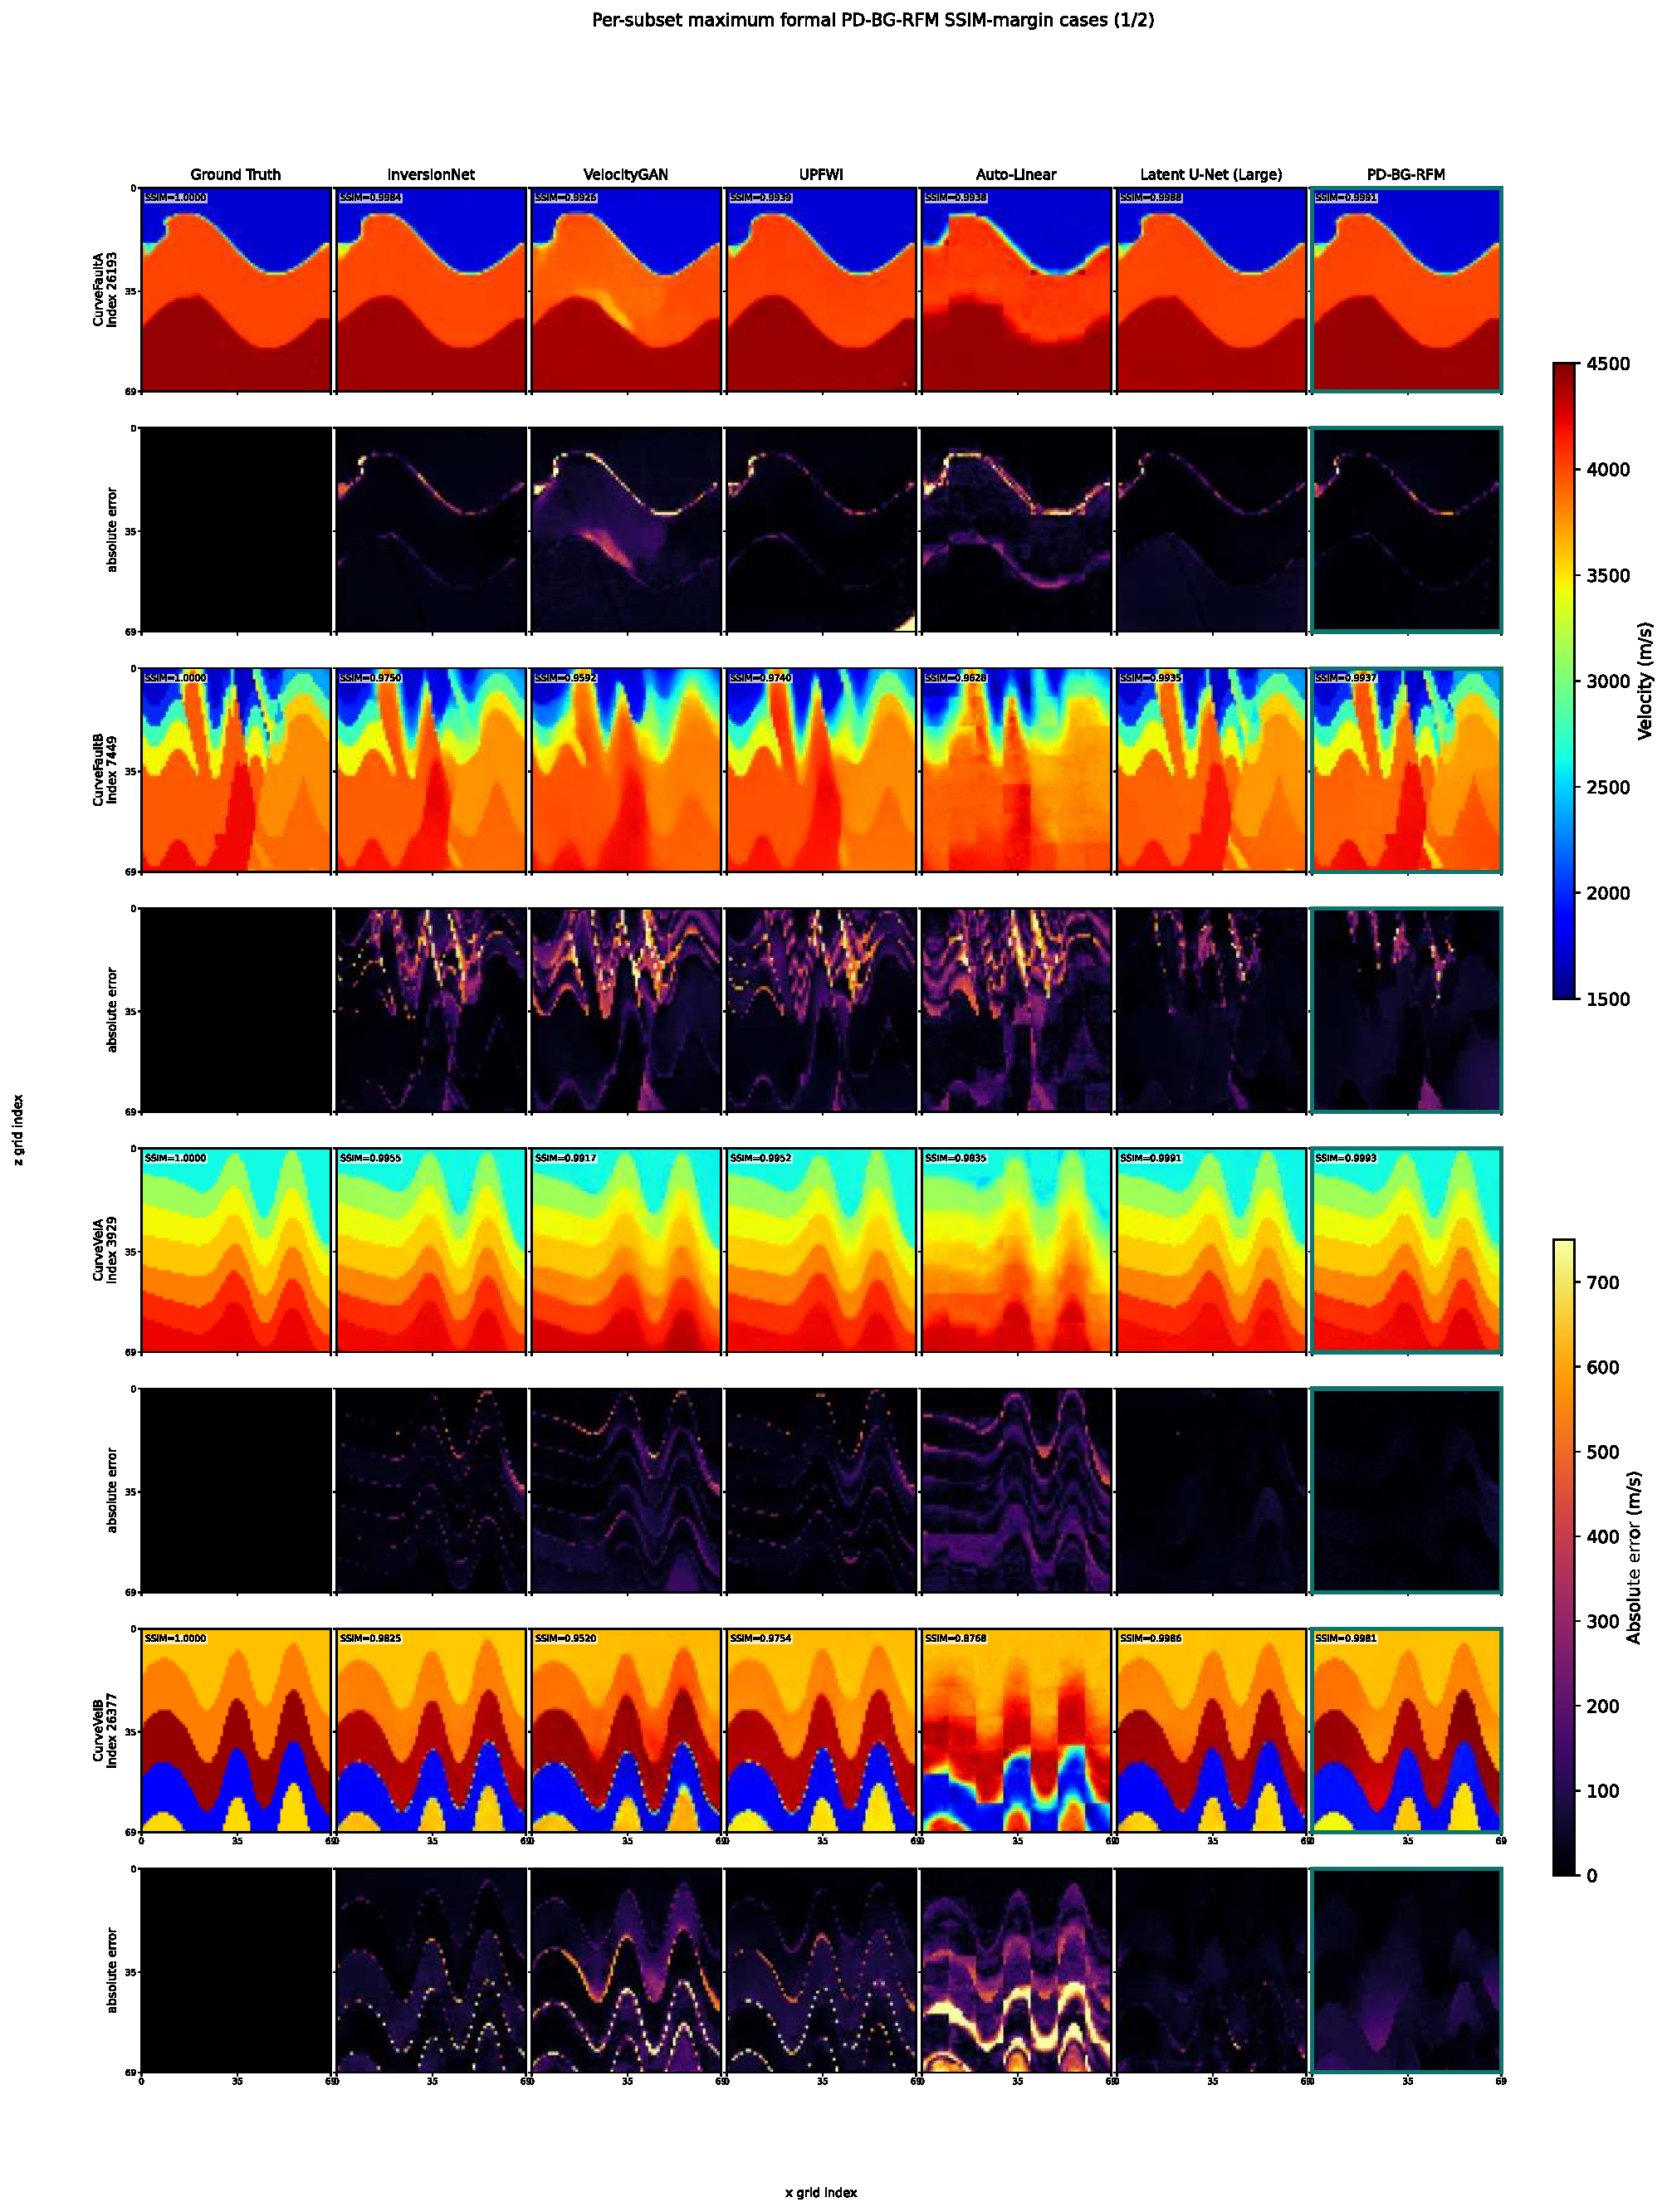
\includegraphics[width=\textwidth,height=0.82\textheight,keepaspectratio]{figures/aaai/table2_representative_cases_1.pdf}
\caption{Fixed-rule qualitative cases for the first four OpenFWI subsets, selected by maximum formal SSIM margin. Display conventions follow Figure~\ref{fig:adapted-qualitative}.}
\label{fig:table2-representative-a}
\end{figure*}

\begin{figure*}[p]
\centering
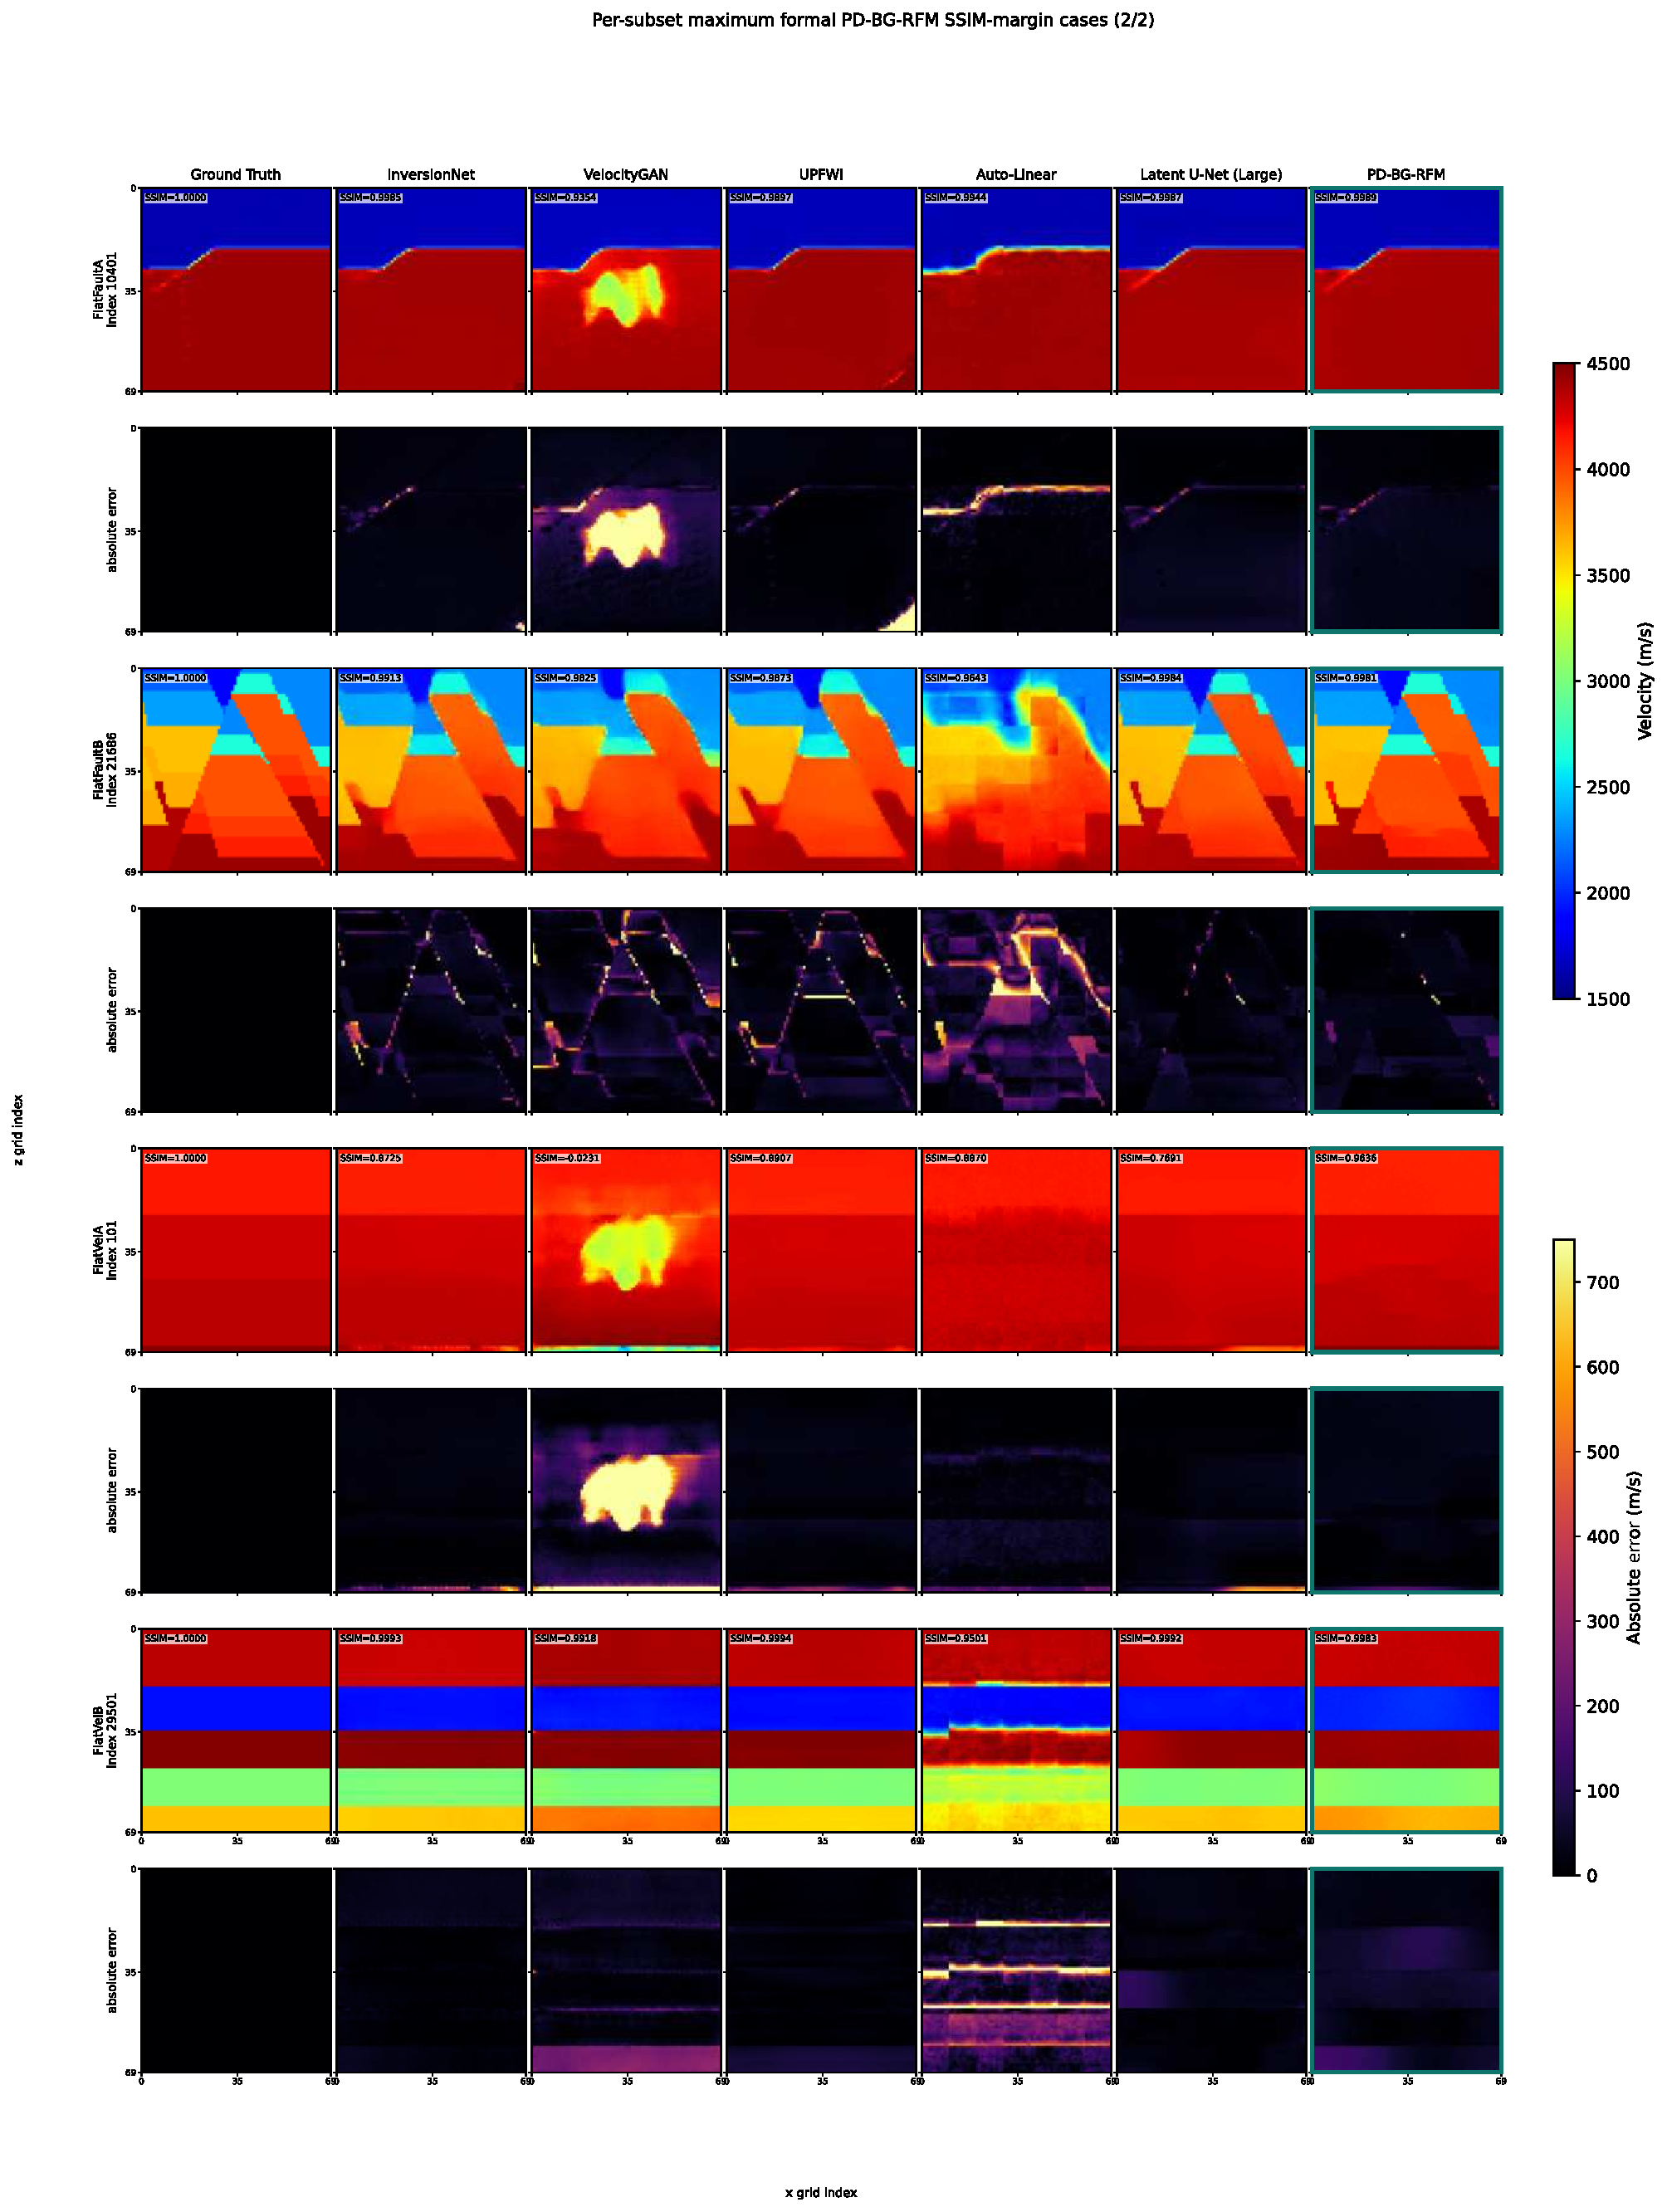
\includegraphics[width=\textwidth,height=0.82\textheight,keepaspectratio]{figures/aaai/table2_representative_cases_2.pdf}
\caption{Fixed-rule qualitative cases for the remaining four OpenFWI subsets under the selection and display conventions of Figure~\ref{fig:table2-representative-a}.}
\label{fig:table2-representative-b}
\end{figure*}

\begin{figure*}[p]
\centering
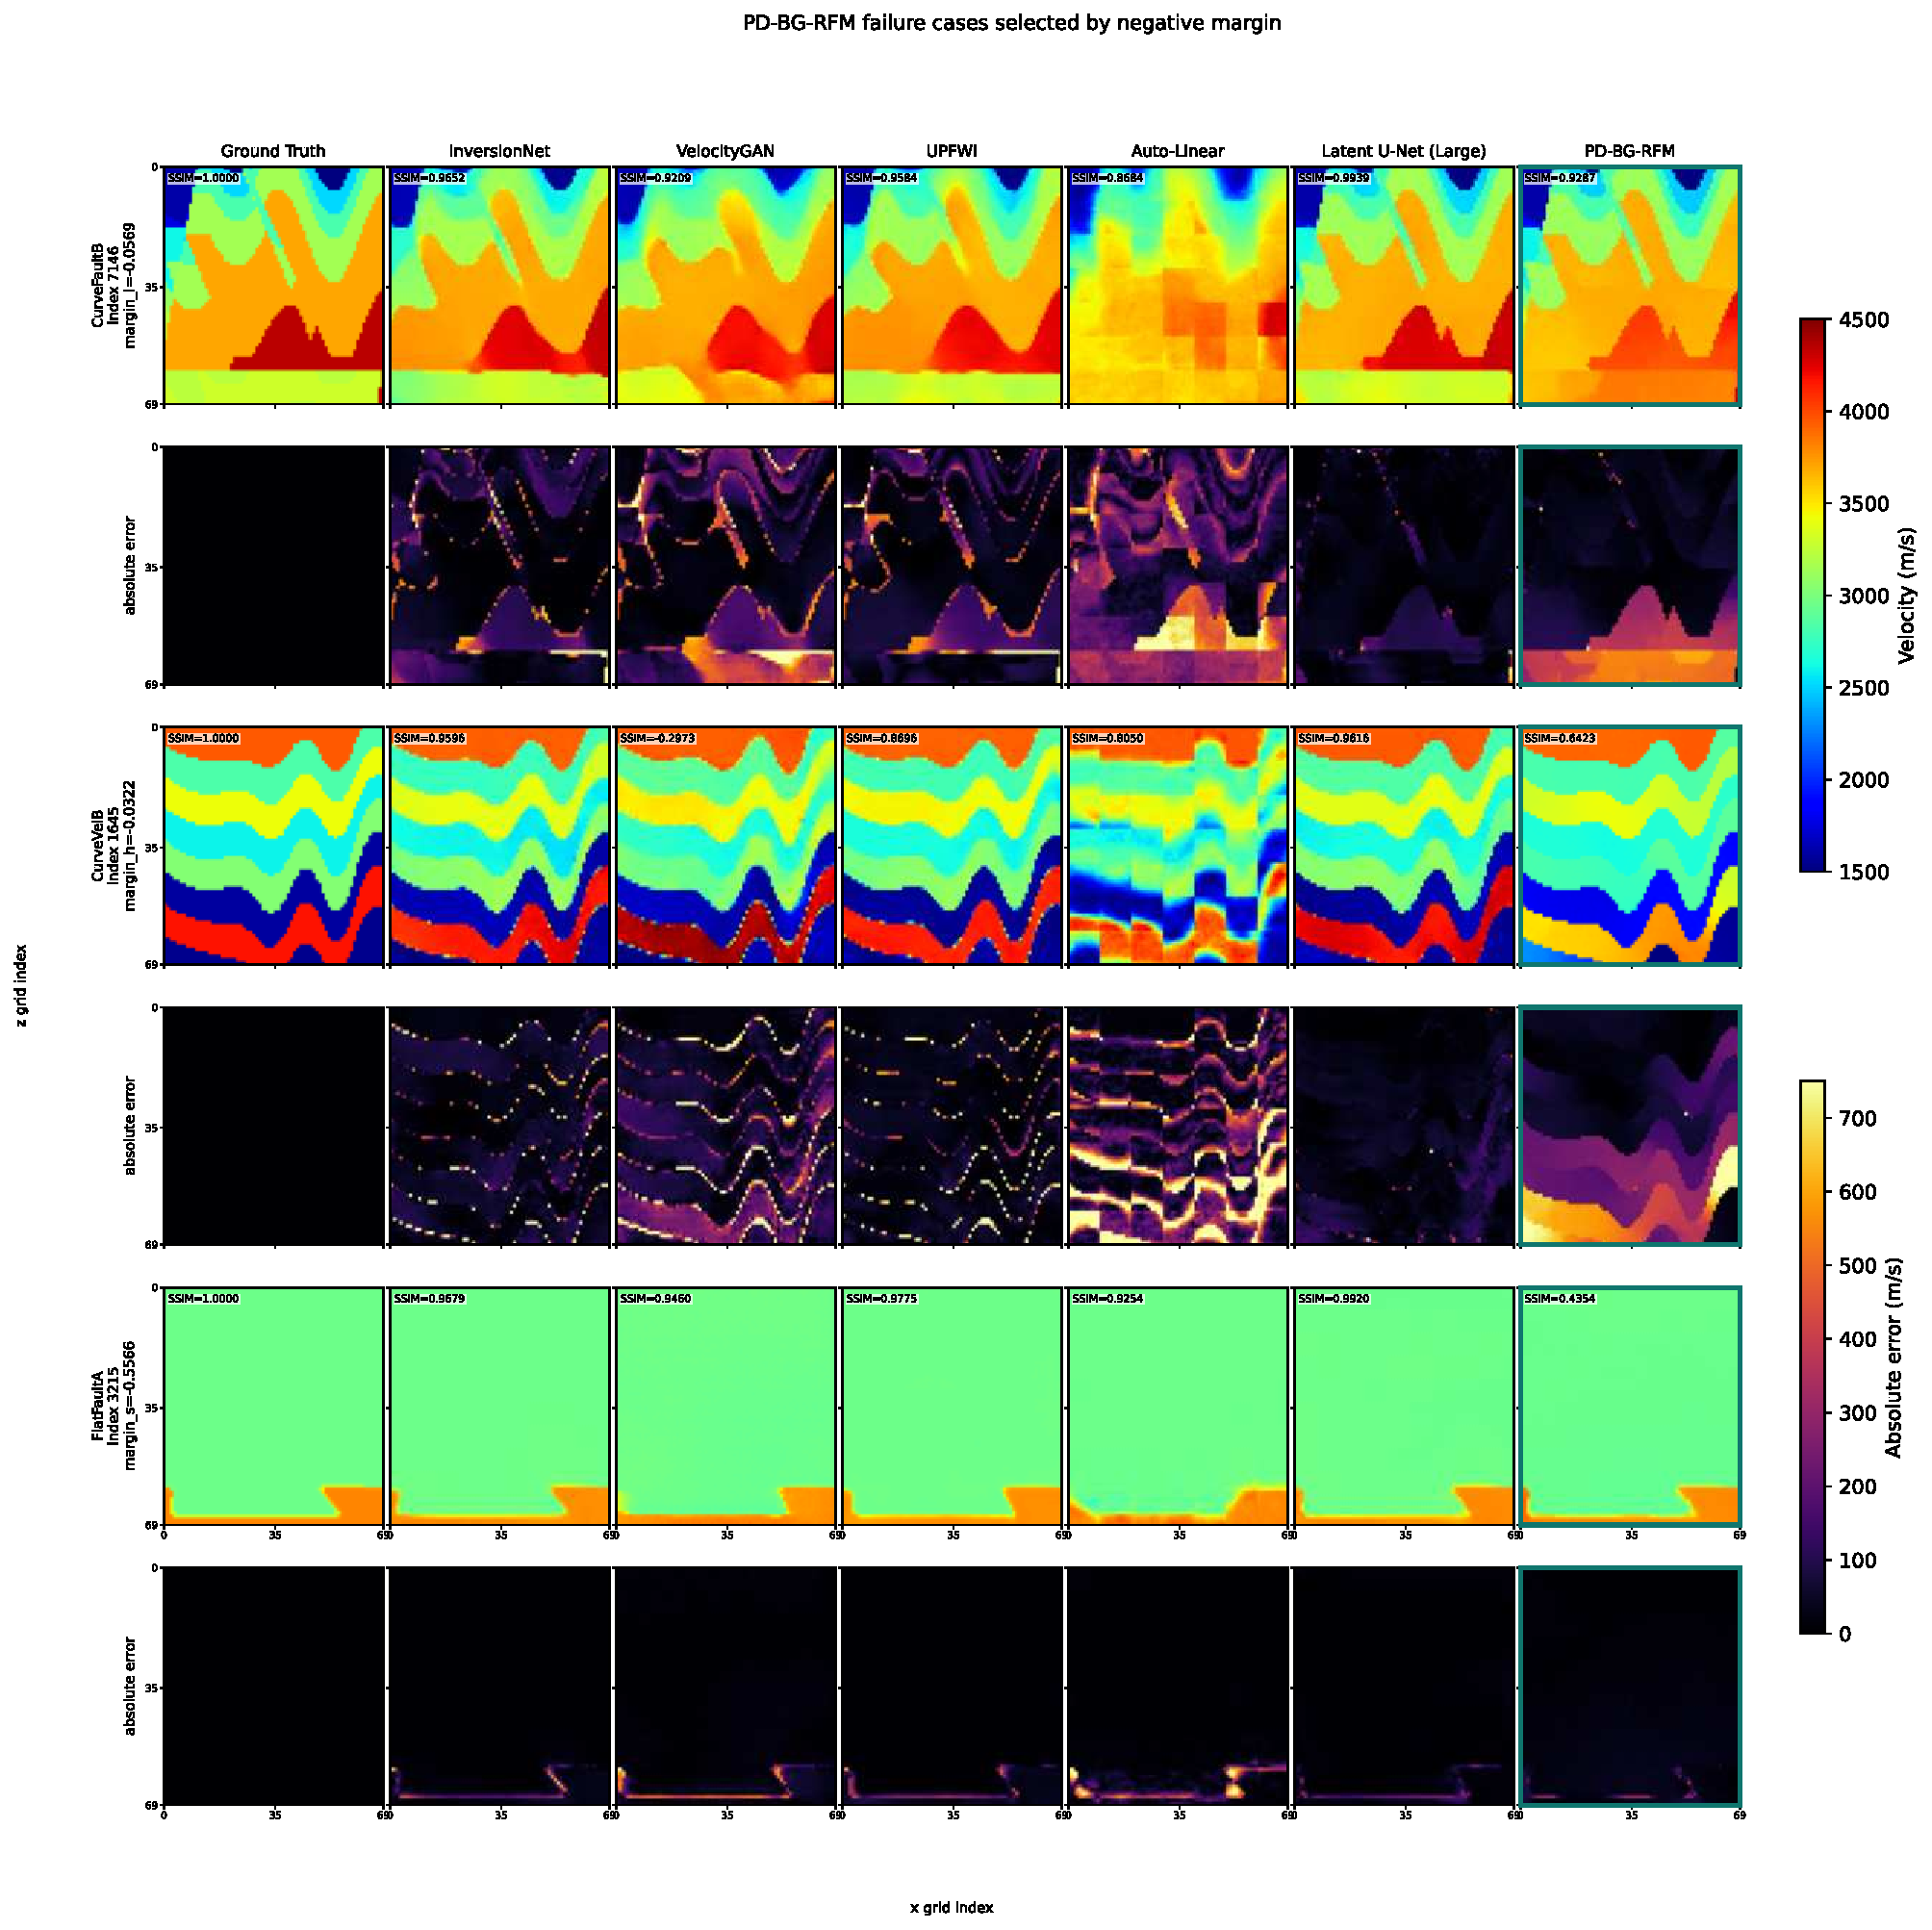
\includegraphics[width=0.99\textwidth]{figures/aaai/table2_failure_cases.pdf}
\caption{Fixed-rule failure cases with the most negative low-frequency, high-frequency, and SSIM margins, respectively.}
\label{fig:table2-failures}
\end{figure*}

\subsection{Additional Component Ablations}
\label{app:component-ablations}
The core attribution table isolates the construction sequence from condition decomposition to background residualization and prediction consistency. The following controls test complementary components without obscuring that chain.
\begin{table}[t]
\centering
\small
\begin{tabular}{@{}p{0.31\columnwidth}@{\hspace{4pt}}p{0.57\columnwidth}@{}}
\toprule
Variant & Isolated factor \\
\midrule
w/o background context & Removes $\psi_{\mathrm{bg}}(\hat B)$ from residual FM. \\
Direct residual predictor & Replaces FM with deterministic residual regression. \\
Uniform fusion & Replaces Eq.~\ref{eq:reliability-fusion} by equal weights over available inputs. \\
w/o condition objective & Sets $\lambda_C=0$ while preserving the routing architecture. \\
\bottomrule
\end{tabular}
\caption{Definitions of additional component controls. They use the data, evaluator, and validation-based checkpoint selection of the core ablations.}
\label{tab:component-ablations}
\end{table}

\subsection{Condition and Transport Diagnostics}
\subsubsection{Condition contract.}
\label{app:condition-diagnostics}
For a feature map $C$, define $M_L(C)=\operatorname{mean}|P_L(C)|$ and $M_H(C)=\operatorname{mean}|P_H(C)|$. The fused-feature diagnostic reports
\begin{align}
\eta_{\mathrm{bg}}&=\frac{M_L(C_{\mathrm{bg}})}{\max(M_L(C_{\mathrm{bg}})+M_H(C_{\mathrm{bg}}),\epsilon)},\\
\eta_{\mathrm{str}}&=\frac{M_H(C_{\mathrm{str}})}{\max(M_L(C_{\mathrm{str}})+M_H(C_{\mathrm{str}}),\epsilon)}.
\end{align}
Larger values indicate stronger agreement with the intended frequency role, but they neither identify the representation nor show that complementary information is absent. Separate squared-energy ratios are retained only for per-modality head diagnostics. We report both diagnostic families with anchor alignment, pairwise retrieval, and visualized condition maps.

\subsubsection{Background-residual transport.}
\label{app:background-diagnostics}
The implementation retains the artifact key \texttt{rho\_B} for backward compatibility, but the paper denotes it by $\rho_{L/H}$. With $d=HW$, the two residual-burden diagnostics are
\begin{align}
\rho_{L/H}
&=\frac{\operatorname{mean}|P_L(V-\hat B)|}
{\operatorname{mean}|P_H(V)|+10^{-6}},\\
e_{R/V}
&=\frac{d^{-1}\|V-\hat B\|_2^2}
{d^{-1}\|V\|_2^2+10^{-8}}.
\end{align}
The first normalizes residual low-pass magnitude by complementary target-detail magnitude, whereas the second measures residual-to-full-field squared energy. We additionally report background MAE, $\epsilon_H^B=\operatorname{mean}|P_H(\hat B)|$, and $q_T$ from Eq.~\ref{eq:transport-diagnostic}. Theorem~1(ii) explains the numerator of $\rho_{L/H}$, while Theorem~1(iii) gives the exact interpretation of $q_T$. These are diagnostics, not training-time gates.

\subsection{Missing-Modality Robustness}
\label{app:missing-modality}
We evaluate a fixed checkpoint with full input, each principal modality removed, both well log and RMS velocity removed, and PoSTM alone. No retraining or test-time adaptation is performed. Absolute metrics measure retained accuracy, while changes from full input quantify degradation as evidence is removed. Reliability weighting is evaluated as an adaptive fusion mechanism rather than a robustness guarantee. These subsets distinguish the loss of sparse calibration from well logs, interpreted structure from horizons, smooth kinematics from RMS velocity, and all auxiliary magnitude-calibrating evidence. PoSTM alone provides the most severe setting and measures how much reconstruction quality remains under structural imaging only.

\begin{table}[t]
\centering
\small
\begin{tabular}{@{}l@{\hspace{8pt}}c@{\hspace{8pt}}c@{\hspace{8pt}}c@{}}
\toprule
Observation subset & MAE & RMSE & SSIM \\
\midrule
Full input & 0.0150 & 0.0269 & 0.9915 \\
w/o well-log & 0.0168 & 0.0295 & 0.9899 \\
w/o horizon & 0.1011 & 0.1669 & 0.8202 \\
w/o RMS velocity & 0.3947 & 0.4705 & 0.0753 \\
w/o well-log + RMS velocity & 0.4684 & 0.5303 & 0.0192 \\
PoSTM only & 0.4706 & 0.5356 & 0.0154 \\
\bottomrule
\end{tabular}
\caption{Missing-modality evaluation of a fixed PD-BG-RFM checkpoint without retraining or test-time adaptation.}
\label{tab:missing-modality}
\end{table}

\section{Complete Condition-Learning Objective}
\label{app:condition-objective}
\subsection{Reliability-Weighted Fusion}
Restoring the sample index suppressed in Eq.~\ref{eq:reliability-fusion}, let $a_{i,m}\in\{0,1\}$ be modality availability, $q_{i,m}\in[0,1]$ its externally supplied quality, and $r_{i,m}^k\in(0,1)$ the predicted reliability for role $k\in\{\mathrm{bg},\mathrm{str}\}$. The fusion weights are
\begin{align}
\widetilde w_{i,m}^k
&=a_{i,m}q_{i,m}r_{i,m}^k,\nonumber\\
w_{i,m}^k
&=\frac{\widetilde w_{i,m}^k}
{\max\!\left(\sum_{m'\in\mathcal M}\widetilde w_{i,m'}^k,\epsilon\right)}.
\label{eq:fusion-normalization}
\end{align}
Here $\epsilon=10^{-6}$ is the numerical stabilizer used for fusion and feature-ratio diagnostics.
The background role uses the numerical reliability channel and the structural role uses the structural channel. In the reported protocol, $q_{i,m}=a_{i,m}$, so quality carries no target-derived information.

\subsection{Subset-Symile and Anchor Calibration}
For role $k\in\{\mathrm{bg},\mathrm{str}\}$, samples are first grouped by their observed subset $\Omega$. We retain a group $\mathcal I_\Omega$ only when $|\Omega|\ge2$ and $|\mathcal I_\Omega|\ge G_{\min}$, with $G_{\min}=2$ in the reported model. Define $\mathcal R_{\Omega,k}=\Omega\cup\{A_k\}$ and let $z^k_{i,r}\in\mathbb R^D$ be its normalized projected representations. Modality projections are multiplied by their within-subset normalized reliability, while $A_k$ is the training-only role anchor. For each held-fixed member $a$ and negative shuffle $j\in\{1,\ldots,J_\Omega\}$, with $J_\Omega=|\mathcal I_\Omega|-1$, the matched and deranged scores are
\begin{align}
s^+_{i,a,k}
&=\sum_{d=1}^{D}\prod_{r\in\mathcal R_{\Omega,k}} z^k_{i,r,d},\\
s^-_{i,a,j,k}
&=\sum_{d=1}^{D}z^k_{i,a,d}
\prod_{r\in\mathcal R_{\Omega,k}\setminus\{a\}}
z^k_{\pi_{a,j,r}(i),r,d},
\end{align}
where every $\pi_{a,j,r}$ is a strict in-group derangement. The implemented role loss is the mean over retained groups, samples, and held-fixed members of
\begin{equation}
-\log
\frac{\exp(s^+_{i,a,k}/\tau)}
{\exp(s^+_{i,a,k}/\tau)+\sum_j\exp(s^-_{i,a,j,k}/\tau)}.
\label{eq:subset-symile-detail}
\end{equation}
Thus the positive tuple is included explicitly in the normalization. Groups below the minimum size contribute zero Subset-Symile loss; missing modalities are excluded rather than replaced by pseudo-observations.

Anchor calibration is computed per role and observed modality. Let $\mathcal I_m$ be the samples containing modality $m$, $\pi_m$ and $\pi_A^k$ be the two-layer modality and role-anchor projection heads, and $\bar r_{m,k}$ be the mean detached reliability over $\mathcal I_m$. Then
\begin{align}
\ell_{m,k}
&=\ell\!\left(\pi_m(Z_m^k[\mathcal I_m]),
\pi_A^k(A_k[\mathcal I_m])\right),\\
\mathcal L_A
&=\frac{1}{2}\sum_{k\in\{\mathrm{bg},\mathrm{str}\}}
\operatorname*{mean}_{m:\,|\mathcal I_m|>0}
\bar r_{m,k}\ell_{m,k},
\end{align}
where $\ell$ is symmetric InfoNCE and falls back to matched cosine distance for a singleton $\mathcal I_m$.

\subsection{Regularization and Diagnostic Terms}
The auxiliary head is $D_m=P_m^U(F_m)$ and is used only in the following separation term. Orthogonality uses pooled cosine magnitude:
\begin{equation}
\mathcal L_{\mathrm{bg,str}}^{\perp}
=\mathbb E_{i,m}|\cos(Z_{i,m}^{\mathrm{bg}},Z_{i,m}^{\mathrm{str}})|,
\end{equation}
with $\mathcal L_{\mathrm{aux}}^{\perp}$ defined analogously between $D_m$ and each routed role. The reliability prior is the mean squared deviation between predicted role reliabilities and fixed modality-role priors over observed inputs. In the reported configuration, $\lambda_A=0.5$ and $\lambda_{\mathrm{bg,str}}=\lambda_{\mathrm{aux}}=\lambda_Q=0.05$. Pairwise contrastive weights and explicit structural-low/background-high penalty weights are zero. Pairwise retrieval and frequency ratios are still computed as diagnostics but do not contribute to gradients through Eq.~\ref{eq:condition-loss}. Let $\mathcal O=\{(i,m):a_{i,m}q_{i,m}>0\}$ denote the observed sample--modality pairs. The reliability prior is
\begin{equation}
\mathcal L_{\mathrm{rel}}
 =\frac{1}{2|\mathcal O|}
 \sum_{(i,m)\in\mathcal O}
 \sum_{k\in\{\mathrm{bg},\mathrm{str}\}}
 \bigl(r_{i,m}^k-\pi_m^k\bigr)^2,
\end{equation}
where $\pi_m^k$ is a fixed modality--role prior.

Together, Subset-Symile, anchor calibration, and orthogonality provide an information-routing interpretation of the active objective, but we do not claim that they form a variational mutual-information bound. Theorem~1 and Corollary~1 do not depend on this interpretation.


\section{Implementation and Evaluation Protocols}
\label{app:implementation}
\subsection{Data and Architecture}
The OpenFWI corpus contains 336,000 examples across the eight subsets used in this work. A deterministic split with seed 42 assigns 235,200 examples to training, 67,200 to validation, and 33,600 to testing. Every target and dense observation is represented on a $70\times70$ grid and normalized to $[-1,1]$. Well-log observations contain zero to three sampled wells per example using well seed 1234, accompanied by an explicit well mask. Missing modalities are represented by a zero availability flag and do not enter Subset-Symile tuples or reliability-weighted fusion.

The encoder uses 32 base channels and produces 16-channel role maps. The background predictor receives the background role map without an additional adapter and is a direct U-Net with 192 hidden channels; the structural role map is projected to 32 channels before entering the 128-channel residual FiLM U-Net. The residual generator operates through an identity codec with one velocity channel. The low-pass operator is stride-one $5\times5$ average pooling. Background supervision uses unit L1 weight and 0.5 L2 weight. Residual training uses unit reconstruction weight and 0.2 low-pass target-matching weight. All L1 and squared-L2 training terms are averaged over batch, channel, and spatial entries. The condition loss uses temperature 0.1, anchor weight 0.5, and weights 0.05 for background/structural orthogonality, auxiliary-head orthogonality, and the reliability prior; its contribution to joint training is scaled by $\lambda_C=0.01$. Pairwise contrastive, condition-space structural-low/background-high penalty, quality-gate, and target-derived gate-loss weights are zero in the reported model.

\subsection{Optimization and Inference}
PD-BG-RFM is trained end-to-end from random initialization. AdamW \cite{loshchilov2019decoupled} uses learning rates $10^{-6}$ for encoder backbones, $3\times10^{-6}$ for encoder heads, contrastive projectors, and adapters, $10^{-4}$ for the background branch, and $5\times10^{-5}$ for the residual branch. Training runs for 100 epochs with a per-process batch size of 64, four-way distributed data parallelism, no gradient accumulation (effective batch size 256), mixed bfloat16 precision, and validation-loss checkpointing. Controlled-ablation checkpoints are selected by validation loss. Residual inference starts from unit Gaussian noise and applies 50 Euler steps. The common evaluator processes every globally selected test record and reports per-sample MAE, RMSE, SSIM, and decomposition diagnostics before micro-aggregation.

\subsection{Run Accounting and Checkpoint Selection}
Split membership is fixed by seed 42, and well locations are generated deterministically from well seed 1234 and the record index. Evaluation traverses the materialized held-out membership with \texttt{shuffle=False}. The formal training configurations do not set \texttt{training.seed}; consequently, model initialization, minibatch order, and Flow Matching noise are not claimed to be bitwise reproducible across retraining. The retained checkpoints and held-out manifests identify the exact reported runs. Each matched-input and ablation row is obtained from one formal training trajectory and one complete evaluation over 33,600 records; resumed jobs are continuations of the same trajectory, not independent repeats. The PD-BG-RFM values in Tables~\ref{tab:main-comparison} and~\ref{tab:adapted-comparison} use the same final-checkpoint trajectory from the fixed 100-epoch schedule. Literature values in Table~\ref{tab:main-comparison} are transcribed from their cited sources rather than rerun. We therefore do not report variation across training seeds or claim a significance test over independent retrainings. The confidence interval for $q_T$ uses 2,000 nonparametric bootstrap resamples with seed 2027.

\subsection{Computing Environment}
The in-house formal jobs were run on a CentOS Linux 8 node (Linux 4.18.0) with two 64-core Hygon C86-4G CPUs, 1.5~TiB host memory, and eight K100\_AI accelerators with 65,520~MiB memory each. PD-BG-RFM and the four-device adaptations use four accelerators; the remaining device counts are listed in Table~\ref{tab:final-optimization}. The retained software environment contains Python 3.10.20, PyTorch 2.7.1 with ROCm/HIP 6.3.25405, Lightning 2.5.2, NumPy 1.24.3, SciPy 1.15.3, and scikit-image 0.25.2.

\subsection{Evaluation Metrics}
Let $e_i=\hat V_i-V_i$ be the normalized error for sample $i$, $d=HW$, and $N$ the number of evaluated records. The common evaluator reports sample-level micro-averages
\begin{align}
\mathrm{MAE}
&=\frac{1}{N}\sum_{i=1}^{N}\frac{\|e_i\|_1}{d},\qquad
\mathrm{RMSE}
=\frac{1}{N}\sum_{i=1}^{N}\sqrt{\frac{\|e_i\|_2^2}{d}},\nonumber\\
\mathrm{MAE}_{k}
&=\frac{1}{N}\sum_{i=1}^{N}\frac{\|P_k(e_i)\|_1}{d},
\qquad k\in\{L,H\}.
\label{eq:evaluation-metrics}
\end{align}
Thus the reported RMSE is the mean of per-sample root-mean-square errors, not the square root of a test-set pooled MSE. For global SSIM, the evaluator computes
\begin{equation}
\mathrm{SSIM}_i=
\frac{(2\mu_{\hat V_i}\mu_{V_i}+C_{1,i})(2\sigma_{\hat V_i,V_i}+C_{2,i})}
{(\mu_{\hat V_i}^2+\mu_{V_i}^2+C_{1,i})(\sigma_{\hat V_i}^2+\sigma_{V_i}^2+C_{2,i})},
\label{eq:global-ssim}
\end{equation}
and averages it over samples. Here $L_i=\max(\max V_i-\min V_i,1)$, $C_{1,i}=(0.01L_i)^2$, and $C_{2,i}=(0.03L_i)^2$; variances and covariance use population normalization. MAE summarizes absolute reconstruction error, RMSE emphasizes larger deviations, SSIM measures whole-model structural agreement, and $\mathrm{MAE}_L$ and $\mathrm{MAE}_H$ localize error under the same $5\times5$ low/high decomposition used by the method. Source-native values in Table~\ref{tab:main-comparison} follow the conversions documented in Appendix~\ref{app:benchmark-accounting}; Tables~\ref{tab:adapted-comparison} and~\ref{tab:ablation} use Eqs.~\ref{eq:evaluation-metrics}--\ref{eq:global-ssim} directly.

\subsection{Hyperparameter Selection}
No exhaustive grid or random search was conducted. Published architectures retain their official-capacity constructors, while method-specific widths and loss weights were finalized from preliminary training/validation runs; test metrics were not used for this choice. Candidate counts and ranges were not logged comprehensively, so the corresponding checklist item remains partial. For formal reporting, Latent U-Net uses its minimum-validation-loss checkpoint, InversionNet, VelocityGAN, UPFWI, and Auto-Linear use the final checkpoints named in Appendix~\ref{app:adapted-accounting}, PD-BG-RFM uses the final checkpoint of its fixed 100-epoch schedule, and controlled ablations use validation-loss selection.


\subsection{Cross-Protocol Literature Context}
\label{app:benchmark-accounting}

Table~\ref{tab:main-comparison} presents a source-native comparison between waveform-based inversion and multimodal constraint integration. The cited methods retain their published waveform-to-velocity protocols, whereas PD-BG-RFM uses the multimodal observation contract defined in this paper. Together, the rows characterize the performance of the two paradigms in their native settings; Table~\ref{tab:adapted-comparison} supplies the controlled matched-input estimator comparison.

\subsubsection{Sources and comparison scope.}
The InversionNet, VelocityGAN, and UPFWI values are transcribed from Table~4 of the NeurIPS 2022 OpenFWI benchmark paper~\cite{deng2022openfwi}. For the supervised methods, we use the rows trained with the $\ell_1$ loss: the columns are therefore labeled InversionNet ($\ell_1$) and VelocityGAN ($\ell_1$). UPFWI is represented by the single unsupervised result reported in that table. The ``Method paper'' row nevertheless cites UPFWI's own ICLR 2022 paper~\cite{jin2022upfwi}; it identifies the method publication rather than changing the provenance of the transcribed values. The Auto-Linear values are reported by its ICML 2024 paper~\cite{feng2024autolinear}, and the Invertible X-Net and Latent U-Net values by the ICLR 2025 GFI paper~\cite{gupta2025gfi}. The PD-BG-RFM entries come from the final checkpoint of the fixed 100-epoch schedule, evaluated after materializing the global eight-subset test split. Its held-out manifest contains 33,600 unique identifiers, with zero train/validation overlap and no missing or extra test records.

\subsubsection{Metric conversion.}
The OpenFWI benchmark reports MAE and MSE on normalized velocity maps~\cite{deng2022openfwi}; we retain its MAE values and compute RMSE as the square root of the reported MSE. Auto-Linear likewise reports normalized MAE and MSE on the $[-1,1]$ velocity scale~\cite{feng2024autolinear}. For both sources,
\begin{equation}
\mathrm{RMSE}_{n}=\sqrt{\mathrm{MSE}_{n}}.
\end{equation}
The GFI paper reports MAE and MSE after mapping predictions to the physical velocity range $[1500,4500]$~m/s~\cite{gupta2025gfi}. Since the half-range of this affine map is $1500$~m/s, the corresponding normalized errors are
\begin{equation}
\mathrm{MAE}_{n}=\frac{\mathrm{MAE}_{\mathrm{phys}}}{1500},
\qquad
\mathrm{RMSE}_{n}=\sqrt{\frac{\mathrm{MSE}_{\mathrm{phys}}}{1500^2}}.
\end{equation}
SSIM values are recorded as reported by the source papers; the PD-BG-RFM column uses the common evaluator's mean per-sample SSIM. Its subset RMSE values are computed as the square root of each subset's pooled MSE, whereas Table~\ref{tab:adapted-comparison} reports mean per-sample RMSE.

\subsubsection{Parameter accounting.}
For the OpenFWI baselines, we use the official repository at commit \texttt{48754806b7b4}, instantiate the network definitions with their default channel widths, and sum all parameters with \texttt{requires\_grad=True}, including affine normalization parameters. InversionNet uses $24{,}409{,}123$ parameters ($24.41$M). VelocityGAN uses the same InversionNet generator with $24{,}409{,}123$ parameters and a discriminator with $1{,}180{,}003$ parameters; the table reports their training-time total, $25{,}589{,}126$ ($25.59$M), while inference uses only the generator. UPFWI is mapped to the official implementation's \texttt{FCN4\_Deep\_Resize\_2} network, which contains $18{,}996{,}259$ trainable parameters ($19.00$M). The UPFWI paper does not directly report this number, so it is explicitly a recomputed implementation count rather than a paper-reported statistic.

For the GFI baselines, we retain the total-model accounting reported in the GFI paper: $35.45$M for Auto-Linear, $26.06$M for Invertible X-Net, and $34.96$M for Latent U-Net (Large). The PD-BG-RFM count is the total trainable parameter count of the current implementation, reported as $10.6$M. All table entries are rounded to two decimal places in millions.

\subsubsection{Paradigm scope.}
The literature rows retain their published waveform-to-velocity protocols, whereas PD-BG-RFM uses the multimodal observation contract defined in this paper. Together, these rows characterize the performance of the two paradigms in their native settings. Matched-input estimator comparison and controlled design attribution are reported in Tables~\ref{tab:adapted-comparison} and~\ref{tab:ablation}, respectively.


\subsection{Matched-Input Baseline Protocol and Qualitative Selection}
\label{app:adapted-accounting}
Table~\ref{tab:adapted-comparison} uses disclosed adaptations of published architectures rather than values copied from their original papers. Each completed adaptation receives the same PoSTM, horizon, RMS-velocity, well-log, and well-mask representation, and predicts the same normalized $70\times70$ velocity target. Its test dataset is constructed with split seed 42 and traversed deterministically with \texttt{shuffle=False}. Every row covers $33{,}600$ evaluations. MAE, per-sample RMSE, per-sample SSIM, $\mathrm{MAE}_L$, and $\mathrm{MAE}_H$ are computed by the common evaluator and averaged over samples; these are sample-level micro-averages, not equal-weight subset macro-averages.

\begin{table*}[t]
\centering
\small
\begin{tabular}{@{}lcccccccc@{}}
\toprule
Method & Objective & Epochs & Batch/GPU & GPUs & Precision & Learning rate & Weight decay & Schedule \\
\midrule
InversionNet & $\ell_1$ & 100 & 64 & 1 & FP32 & $10^{-4}$ & $10^{-4}$ & none \\
VelocityGAN & GAN+$\ell_1$ & 100 & 64 & 1 & FP32 & $10^{-4}$ (G/D) & $10^{-4}$ & none \\
UPFWI & $\ell_1$ & 100 & 64 & 1 & FP32 & $10^{-4}$ & $10^{-4}$ & none \\
Latent U-Net & $\ell_1$ & 100 & 300 & 4 & bfloat16 & $10^{-4}$ & 0 & none \\
Auto-Linear & AE/inverse & $100+100$ & 128/64 & 4 & bfloat16 & $10^{-4}/10^{-3}$ & 0.05 & cosine \\
PD-BG-RFM & Eq.~\ref{eq:total-loss} & 100 & 64 & 4 & bfloat16 & grouped & 0 & none \\
\bottomrule
\end{tabular}
\caption{Final optimization settings for the matched-input comparison. Batch size is per device; no run uses gradient accumulation.}
\label{tab:final-optimization}
\end{table*}

All rows use AdamW. VelocityGAN uses $(\beta_1,\beta_2)=(0,0.9)$, five discriminator updates per generator update, and weights 100, 1, 10, and 0 for its $\ell_1$, adversarial, gradient-penalty, and MSE terms, respectively. Latent U-Net uses 128 latent channels, depth two, two repeated blocks per level, and skip connections. Auto-Linear uses mask ratio 0.75 and converter rank 375; the first and second entries in its epoch, batch, and learning-rate columns correspond to autoencoder pretraining and inverse translation. The grouped PD-BG-RFM rates and all active loss weights are specified in Appendix~\ref{app:implementation}. InversionNet and UPFWI preserve the official-capacity architectures and use direct $\ell_1$ supervision after replacing only the input interface.

\subsubsection{Architecture adaptations and checkpoints.}
The official-capacity InversionNet, VelocityGAN, and UPFWI implementations are adapted to the five-channel multimodal input while preserving their respective network structures. Their evaluated models have $24{,}409{,}123$, $25{,}589{,}126$ (generator plus discriminator), and $18{,}996{,}259$ reported parameters, respectively.

The latent row adapts GFI's large latent U-Net translation architecture~\cite{gupta2025gfi} and uses a validation-selected checkpoint with $35{,}123{,}429$ active parameters.

Auto-Linear~\cite{feng2024autolinear} is adapted to the same multimodal input while retaining its staged training design; its active inference architecture has $35{,}470{,}032$ parameters.

The proposed-method row uses the final checkpoint from the fixed 100-epoch schedule on the materialized global eight-subset test membership. The held-out manifest contains 33,600 unique records with zero train/validation overlap. Inference uses 50 Euler steps, and the complete trainable model contains approximately $10.6$M parameters.

\subsubsection{Qualitative selection.}
The qualitative panels use the same manifest-backed held-out records as the proposed-method reference row. The three main-text cases are selected without visual inspection: formal per-record metrics rank candidates for each criterion, and deterministic re-inference must preserve the corresponding positive margin against every adapted reference. Figures~\ref{fig:table2-representative-a}--\ref{fig:table2-representative-b} contain one record from each OpenFWI subset maximizing $\mathrm{SSIM}_{\mathrm{PD\text{-}BG\text{-}RFM}}-\max_m\mathrm{SSIM}_m$ over the five adapted references, even when that maximum is non-positive. Figure~\ref{fig:table2-failures} shows the most negative fixed-rule low-frequency, high-frequency, and SSIM margins. All predictions are re-inferred from the formal checkpoints and displayed on a shared physical velocity range.

\fi

\end{document}
